\documentclass[11pt,letterpaper]{article}

\usepackage[T1]{fontenc}
\usepackage[spanish,es-nodecimaldot]{babel}
\usepackage[margin=2.5cm]{geometry}
\usepackage{amsmath,amssymb}
\usepackage{enumitem}
\usepackage{graphicx}
\usepackage[hidelinks]{hyperref}
\usepackage{multicol}
\usepackage{listings}
\emergencystretch=3em
\raggedbottom

\usepackage{csquotes}

\usepackage{caption}
\usepackage{subcaption}
\captionsetup{hypcap=false}

\usepackage{tikz}
\usetikzlibrary{positioning}
\usetikzlibrary{arrows.meta}

\usepackage[
    backend=biber,
    style=authoryear,
    natbib=true,
    maxcitenames=2,
    uniquelist=false
]{biblatex}

\addbibresource{bibliografia.bib}

% Bibliografía en bandera para evitar líneas sueltas (underfull) en columna angosta
\renewcommand*{\bibfont}{\normalfont\raggedright}

% "Cuadro" -> "Tabla" en los captions (babel spanish usa "Cuadro" por defecto)
\addto\captionsspanish{\renewcommand{\tablename}{Tabla}}

% Referencias cruzadas consistentes y automaticas.
% cleveref debe cargarse despues de hyperref.
\usepackage[nameinlink,noabbrev]{cleveref}
\crefname{figure}{Fig.}{Figs.}
\Crefname{figure}{Fig.}{Figs.}
\crefname{equation}{Eq.}{Eqs.}
\Crefname{equation}{Eq.}{Eqs.}
\crefname{table}{Tabla}{Tablas}
\Crefname{table}{Tabla}{Tablas}
% Mostrar el numero de ecuacion sin parentesis (Eq. 1 en vez de Eq. (1))
\creflabelformat{equation}{#2#1#3}

\title{
    Investigación N\textsuperscript{o} 1 RM3100 \\
    \large Información sobre el sensor y conceptos claves
}

\author{Yerko Jelcic Iturra}
\date{\today}

\begin{document}

\maketitle

\begin{abstract}
    El sensor RM3100 es un magnetómetro de tres ejes basado en tecnología magneto-inductiva (MI). A diferencia de los sensores de efecto Hall o magnetorresistivos (RM), no mide un voltaje analógico proporcional al campo, sino que traduce el campo magnético a una frecuencia de oscilación que se cuantifica digitalmente. Esto otorga un ruido bajo (piso de ruido de $4pT/\sqrt{Hz}$ a $1Hz$), salida inherentemente digital sin acondicionamiento analógico, y ausencia de deriva de offset (bias drift) apreciable con la temperatura. El sistema completo consta de tres bobinas sensoras \textbf{(2 Sen-xy, 1 Sen-z)} y un ASIC controlador denominado \textbf{MagI2C}, que excita las bobinas y realiza el conteo temporal.
\end{abstract}

\begin{multicols*}{2}
\section{Principio físico}
El RM3100 pertenece a la familia de sensores magneto-inductivos (MI), el cual, a diferencia de un fluxgate o un sensor de efecto Hall, no mide una tensión proporcional al campo, sino que traduce el campo externo en una variación de inductancia, y de ahí en una variación temporal que un contador digital puede leer directamente. 
El sensor es una bobina solenoidal de $N$ vueltas y longitud $l$, tal que se tiene $n = N/l$ vueltas por unidad de longitud, devanada sobre un núcleo de alta permeabilidad. Aplicando la ley de Ampere para la intensidad del campo $\vec{H}$, que solo depende de las corrientes de conducción, el campo que la propia bobina establece a lo largo del eje es $H_{bob} = \dfrac{N}{l}I = n I$. Por superposición con la componente axial del campo externo $\vec{H}_E$, el núcleo experimenta
\begin{equation}
    H = k_0I + H_E \qquad k_0\equiv n = \dfrac{N}{l}
    \label{eq:1}
\end{equation}
La constante $k_0$ es geométrica y no depende de la permeabilidad. Además, se trabaja en $H$, y no en $B$, para mantener esta parte de la cadena libre de la no linealidad del material \citep{leuzinger2010}.
Sin embargo, el comportamiento del núcleo se describe por su curva de magnetización $B(H)$, mostrada esquemáticamente en la \cref{fig:curva-bh}. En un material ferromagnético blando, esta curva es no lineal, ya que para campos pequeños la respuesta es casi lineal (región de máxima pendiente), luego aparece una curva y finalmente el material satura en $\pm B_s$, donde un incremento de $\vec{H}$ casi no afecta a $\vec{B}$.

De esto, conviene distinguir dos permeabilidades:
\begin{itemize}
    \item Permeabilidad de amplitud: $\mu = \dfrac{B}{H}$
    \item Permeabilidad incremental: $\mu_{inc} = \dfrac{dB}{dH}$
\end{itemize}

La primera corresponde a una relación estática entre B y H, ya que corresponde a la pendiente de la línea que va desde el origen hasta un cierto punto del ciclo de la histéresis para un valor dado de H. En cambio, la segunda representa la pendiente local de una cierta zona del bucle menor para un valor de intensidad de campo dado. A niveles bajos de excitación, la permeabilidad incremental es igual a la permeabilidad inicial. Aumenta el valor de H hasta alcanzar un máximo y, a medida que el nivel de excitación aumenta, el núcleo se satura y la permeabilidad incremental se aproxima a la del vacío \citep{permeability}. Para las pequeñas oscilaciones de corriente que ocurren en el sensor alrededor de un punto de operación, la inductancia dependerá de $\mu_{inc}$ y no de $\mu$.

En la \cref{fig:curva-bh}, $\mu_{inc}$ es máxima cerca del origen y disminuye hacia la saturación. En un núcleo blando, la curva $B(H)$ es prácticamente \textit{anhisterética} (sin lazo de histéresis apreciable) y de simetría impar, $B(-H) = -B(H)$. Para el caso del sensor, el fabricante reporta la ausencia de la histéresis, que es la razón física por la que no presenta deriva de offset apreciable.

\begin{center}
    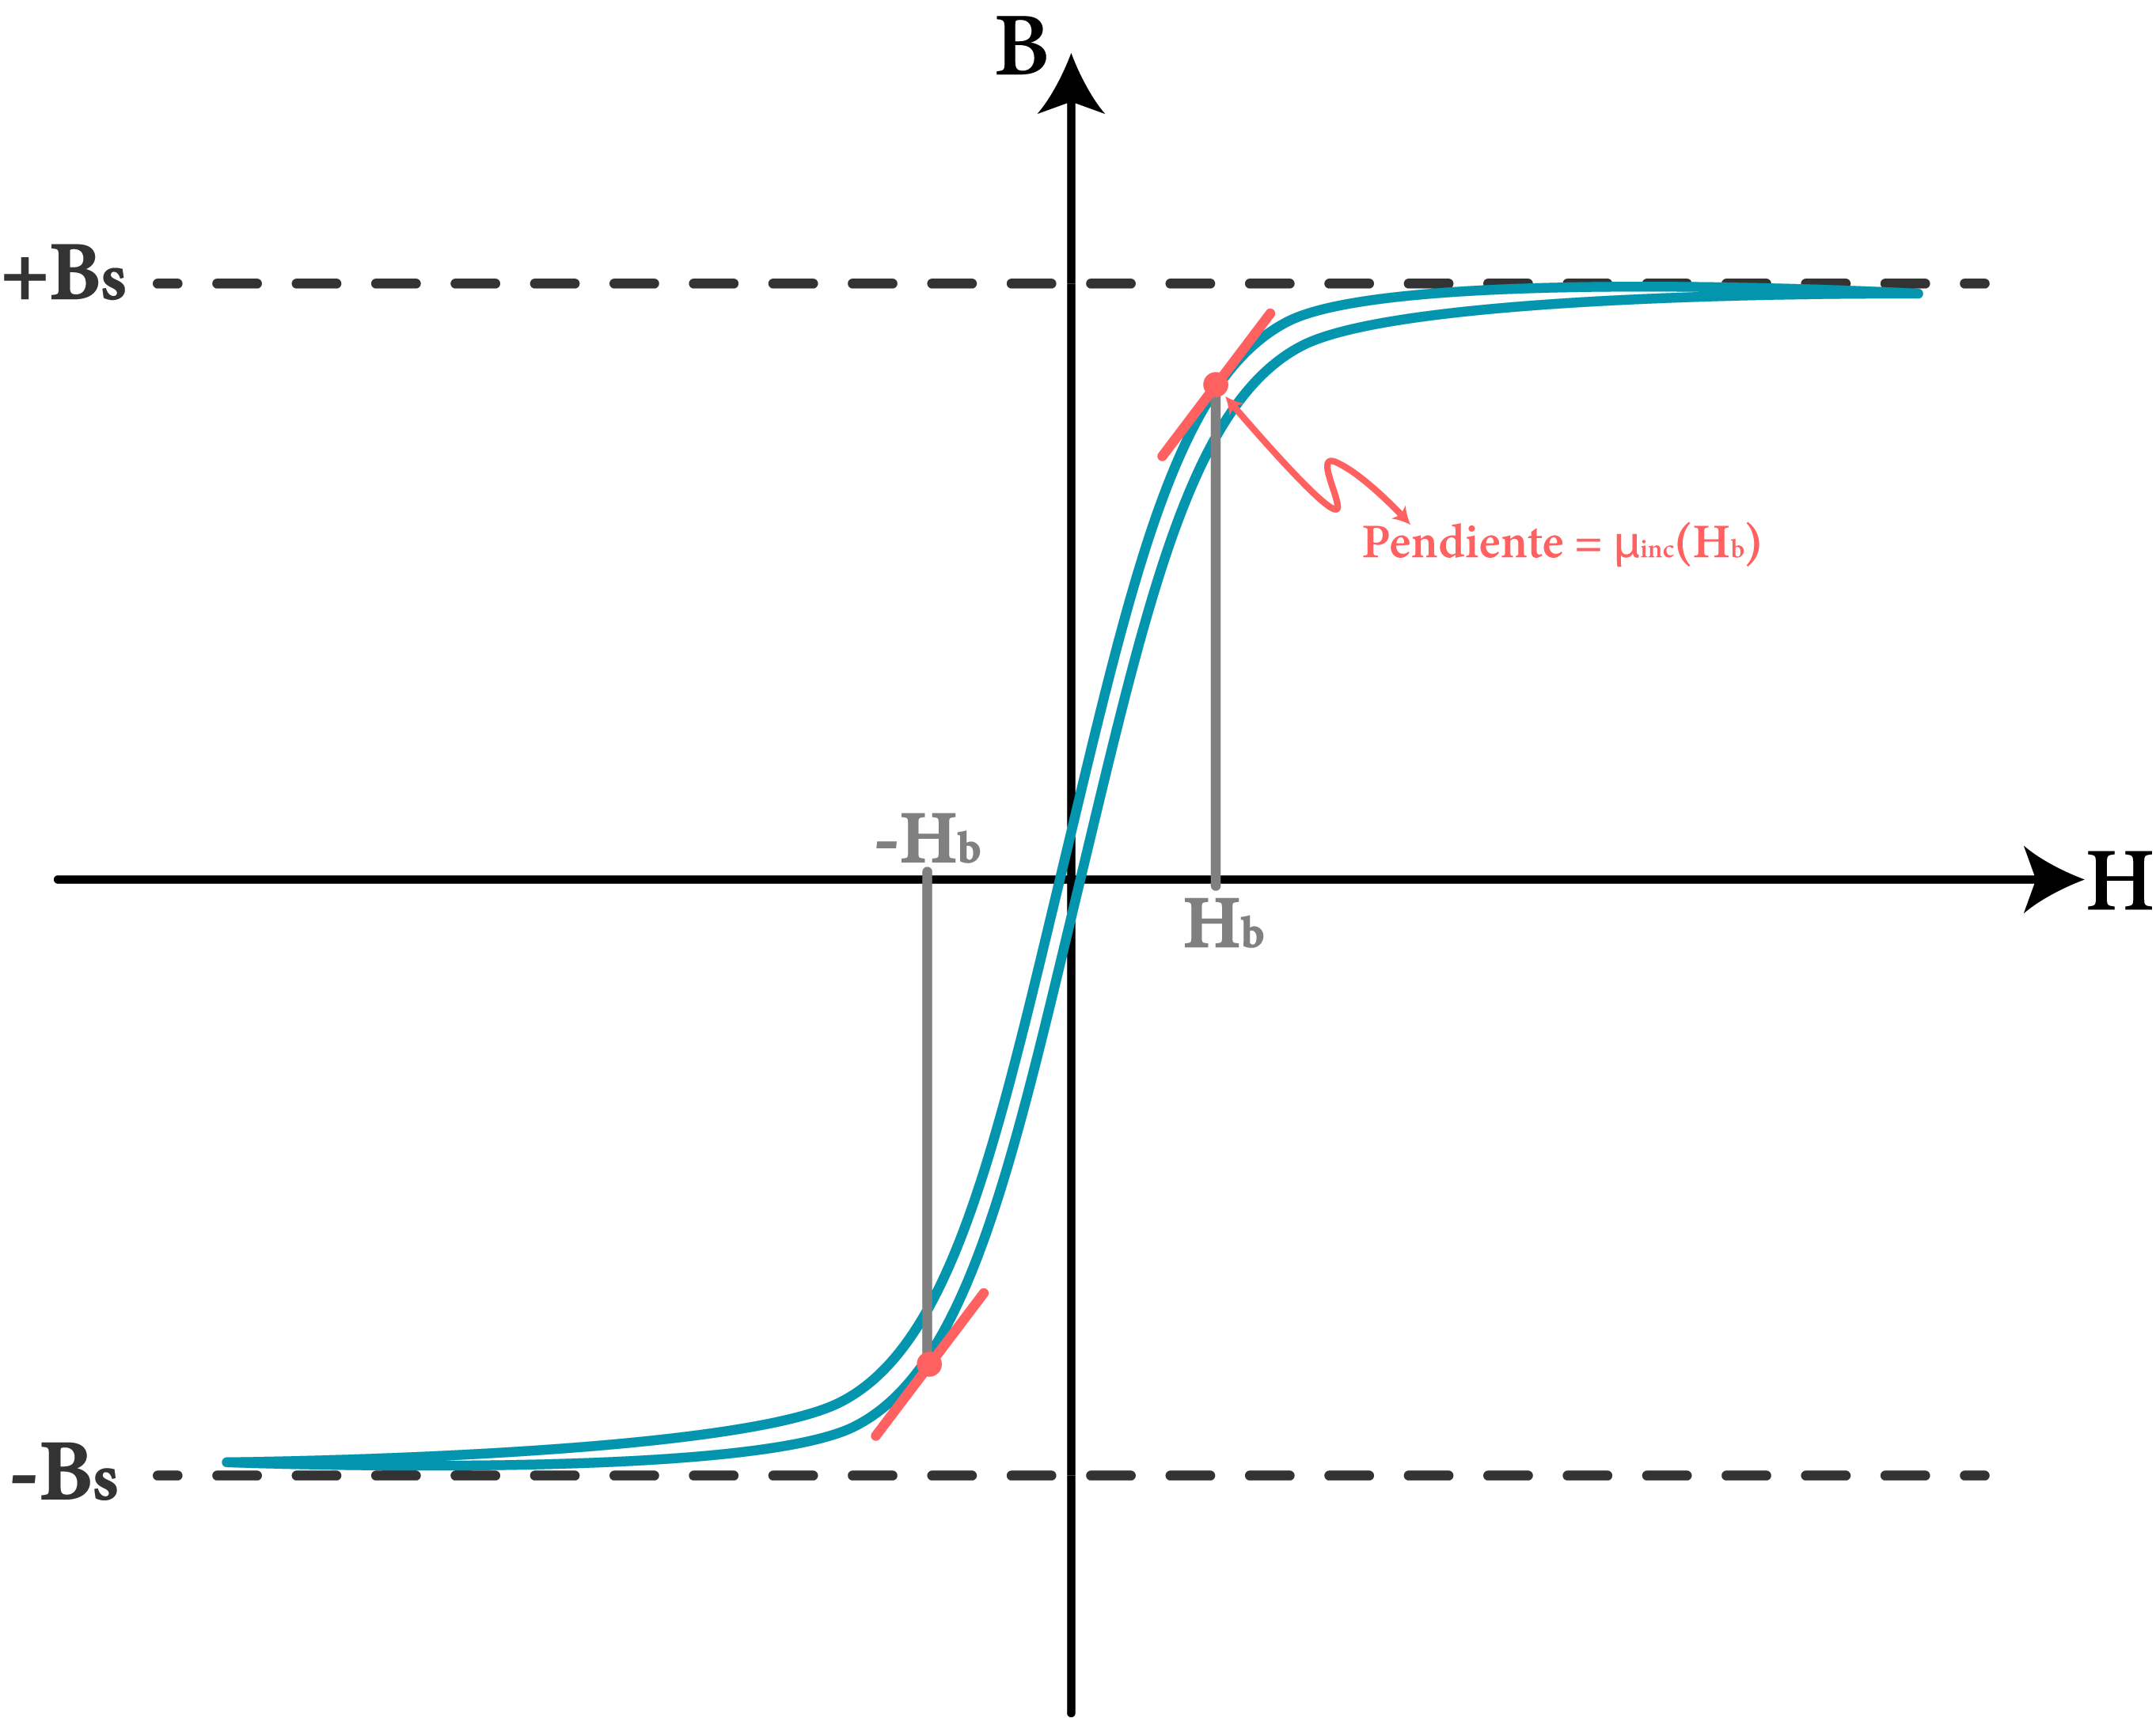
\includegraphics[width=0.9\columnwidth]{assets/curva_B-H.png}
    \captionof{figure}{Curva de magnetización B(H) de un núcleo ferromagnético blando. La permeabilidad incremental $\mu_{inc} = dB/dH$ es la pendiente local; en los puntos de operación $\pm H_b$ (región no lineal) la pendiente cambia con el campo, lo que da sensibilidad al sensor.}
    \label{fig:curva-bh}
\end{center}

Por otro lado, la inductancia se define como la relación entre el diferencial de flujo magnético $Nd\Phi = N\ A \ dB$ y la variación de corriente $I$, donde $N$ corresponde al número de vueltas de la bobina, $B$ es la densidad del flujo magnético y $A$ es el área de la sección transversal. Además, usando la definición de la \cref{eq:1}, se obtiene que:
\begin{align}
    L = N\frac{d\Phi}{dI} &= NA\frac{dB}{dI} \notag \\[2pt]
  = NA\frac{dB}{dH}\frac{dH}{dI} &= NA\mu_{\mathrm{inc}}k_0 \notag \\[2pt]
  = \boxed{\frac{N^2A}{l}\mu_{\mathrm{inc}}(H)} &\equiv G\,\mu_{\mathrm{inc}}(H)
  \label{eq:2}
\end{align}

La inductancia es el factor geométrico G multiplicado por la permeabilidad incremental evaluada en el punto de operación. Por lo tanto, un cambio en el campo externo $H_E$ desplaza el punto de operación sobre la curva B-H (\cref{eq:1}), cambia la pendiente local $\mu_{inc}$ y, con ella, la inductancia (\cref{eq:2}). Esta cadena se resume en la \cref{fig:efecto_campo_inductancia}.

\begin{center}
    
    \begin{tikzpicture}[
            block/.style={
                draw,
                rounded corners,
                align=center,
                minimum width=6cm,
                minimum height=1cm
            }
        ]

        \node[block, fill = blue!30] (campo) {Corriente de excitación $I$ \\y Campo externo $H_{\mathrm{ext}}$};
        
        \node[block, below = 0.8cm of campo] (campo total)
            {Campo total en el núcleo\\
            $H = k_0 I + H_E$};

        \node[block, below = 0.8cm of campo total] (punto)
            {Desplazamiento del punto de\\
            operación en la curva \textit{B-H}};

        \node[block, below = 0.8cm of punto] (permeabilidad)
            {Cambio en la $\mu_{\mathrm{inc}}$\\
            $\displaystyle \mu_{\mathrm{inc}}=dB/dH$};

        \node[block, below = 0.8cm of permeabilidad] (inductancia sensor)
            {Inductancia del sensor\\
            $L = G \mu_{inc}$};
        
        \node[block, below = 0.8cm of inductancia sensor] (relajacion)
            {Constante de relajación\\
            $\tau = L/R_b$};


        \node[block, below = 0.8cm of relajacion, fill = blue!30] (medicion)
            {Medida diferencial\\
            $\Delta t = t_+ - t_- \varpropto H_E$};

        \draw[-{Stealth}, thick] (campo) -- (campo total);
        \draw[-{Stealth}, thick] (campo total) -- (punto);
        \draw[-{Stealth}, thick] (punto) -- (permeabilidad);
        \draw[-{Stealth}, thick] (permeabilidad) -- (inductancia sensor);
        \draw[-{Stealth}, thick] (inductancia sensor) -- (relajacion);
        \draw[-{Stealth}, thick] (relajacion) -- (medicion);


    \end{tikzpicture}
    \captionof{figure}{Cadena física de conversión del sensor magneto-inductivo. El campo externo modifica el punto de operación del núcleo, la permeabilidad incremental y la inductancia. Esto se ve reflejado en el oscilador de relajación, que traduce esa inductancia en tiempos, y la diferencia entre polaridad es proporcional a $H_E$.}
    \label{fig:efecto_campo_inductancia}
\end{center}

\subsection{Oscilador L/R}
El sensor consiste en una conexión en serie con un resistor de bias (polarización de un campo magnético de referencia, conocido y controlado, que el circuito aplica deliberadamente al núcleo para fijar su punto de operación en un lugar elegido de la curva B-H) $R_b$. Aplicando la ley de Kirchhoff, se obtiene de la \cref{fig:circuito-RL}, la siguiente ecuación diferencial del circuito

\begin{align}
    V_S &= V_L + V_R \notag \\
    &= L\dfrac{dI}{dt} + R_b I
\end{align}

donde $V_S$ es el voltaje del Schmitt Trigger. Resolviendo esto, se obtiene que:

\begin{align}
    \dfrac{dI}{dt}
        &= \dfrac{V_S - R_b I}{L} \notag\\
        &= -\dfrac{R_b}{L}\left(I - \dfrac{V_S}{R_b}\right) \notag\\
        &= -\dfrac{R_b}{L}\left(I - I_{\infty}\right) \notag\\
    \intertext{El equilibrio ($dI/dt = 0$) define $I_{\infty} = V_S/R_b$. Con $x = I - I_{\infty}$ (luego $dx = dI$):}
    \dfrac{dx}{dt}
        &= -\dfrac{R_b}{L}\,x \notag\\
    \dfrac{dx}{x}
        &= -\dfrac{R_b}{L}\,dt \quad \Big/\!\int \notag\\
    \ln(x)
        &= -\dfrac{t}{\tau} + \ln(C), \quad \tau = \dfrac{L}{R_b} \notag\\
    \Longrightarrow\ x
        &= C\,e^{-t/\tau} \notag\\
    \intertext{Deshaciendo el cambio y aplicando $I(0) = I_0$:}
    I - I_{\infty}
        &= C\,e^{-t/\tau} \notag\\
    I(t)
        &= I_{\infty} + C\,e^{-t/\tau} \notag\\
    I_0
        &= I_{\infty} + C
         \ \Longrightarrow\ C = I_0 - I_{\infty} \notag\\
    \Longrightarrow
        &\  \boxed{I(t) = \,I_{\infty} + (I_0 - I_{\infty})\,e^{-t/\tau}\,}
    \label{eq:3}
\end{align}
de la \cref{eq:3} aparece la constante de tiempo de relajación
\begin{equation}
    \tau = \dfrac{L}{R_b}
    \label{eq:4}
\end{equation}
Como $L=L(H)$ por la \cref{eq:2}, entonces $\tau = \tau(H)$, es decir, medir el tiempo de relajación es medir, en cierta relación, la inductancia, y por lo tanto, el campo.

\begin{center}
    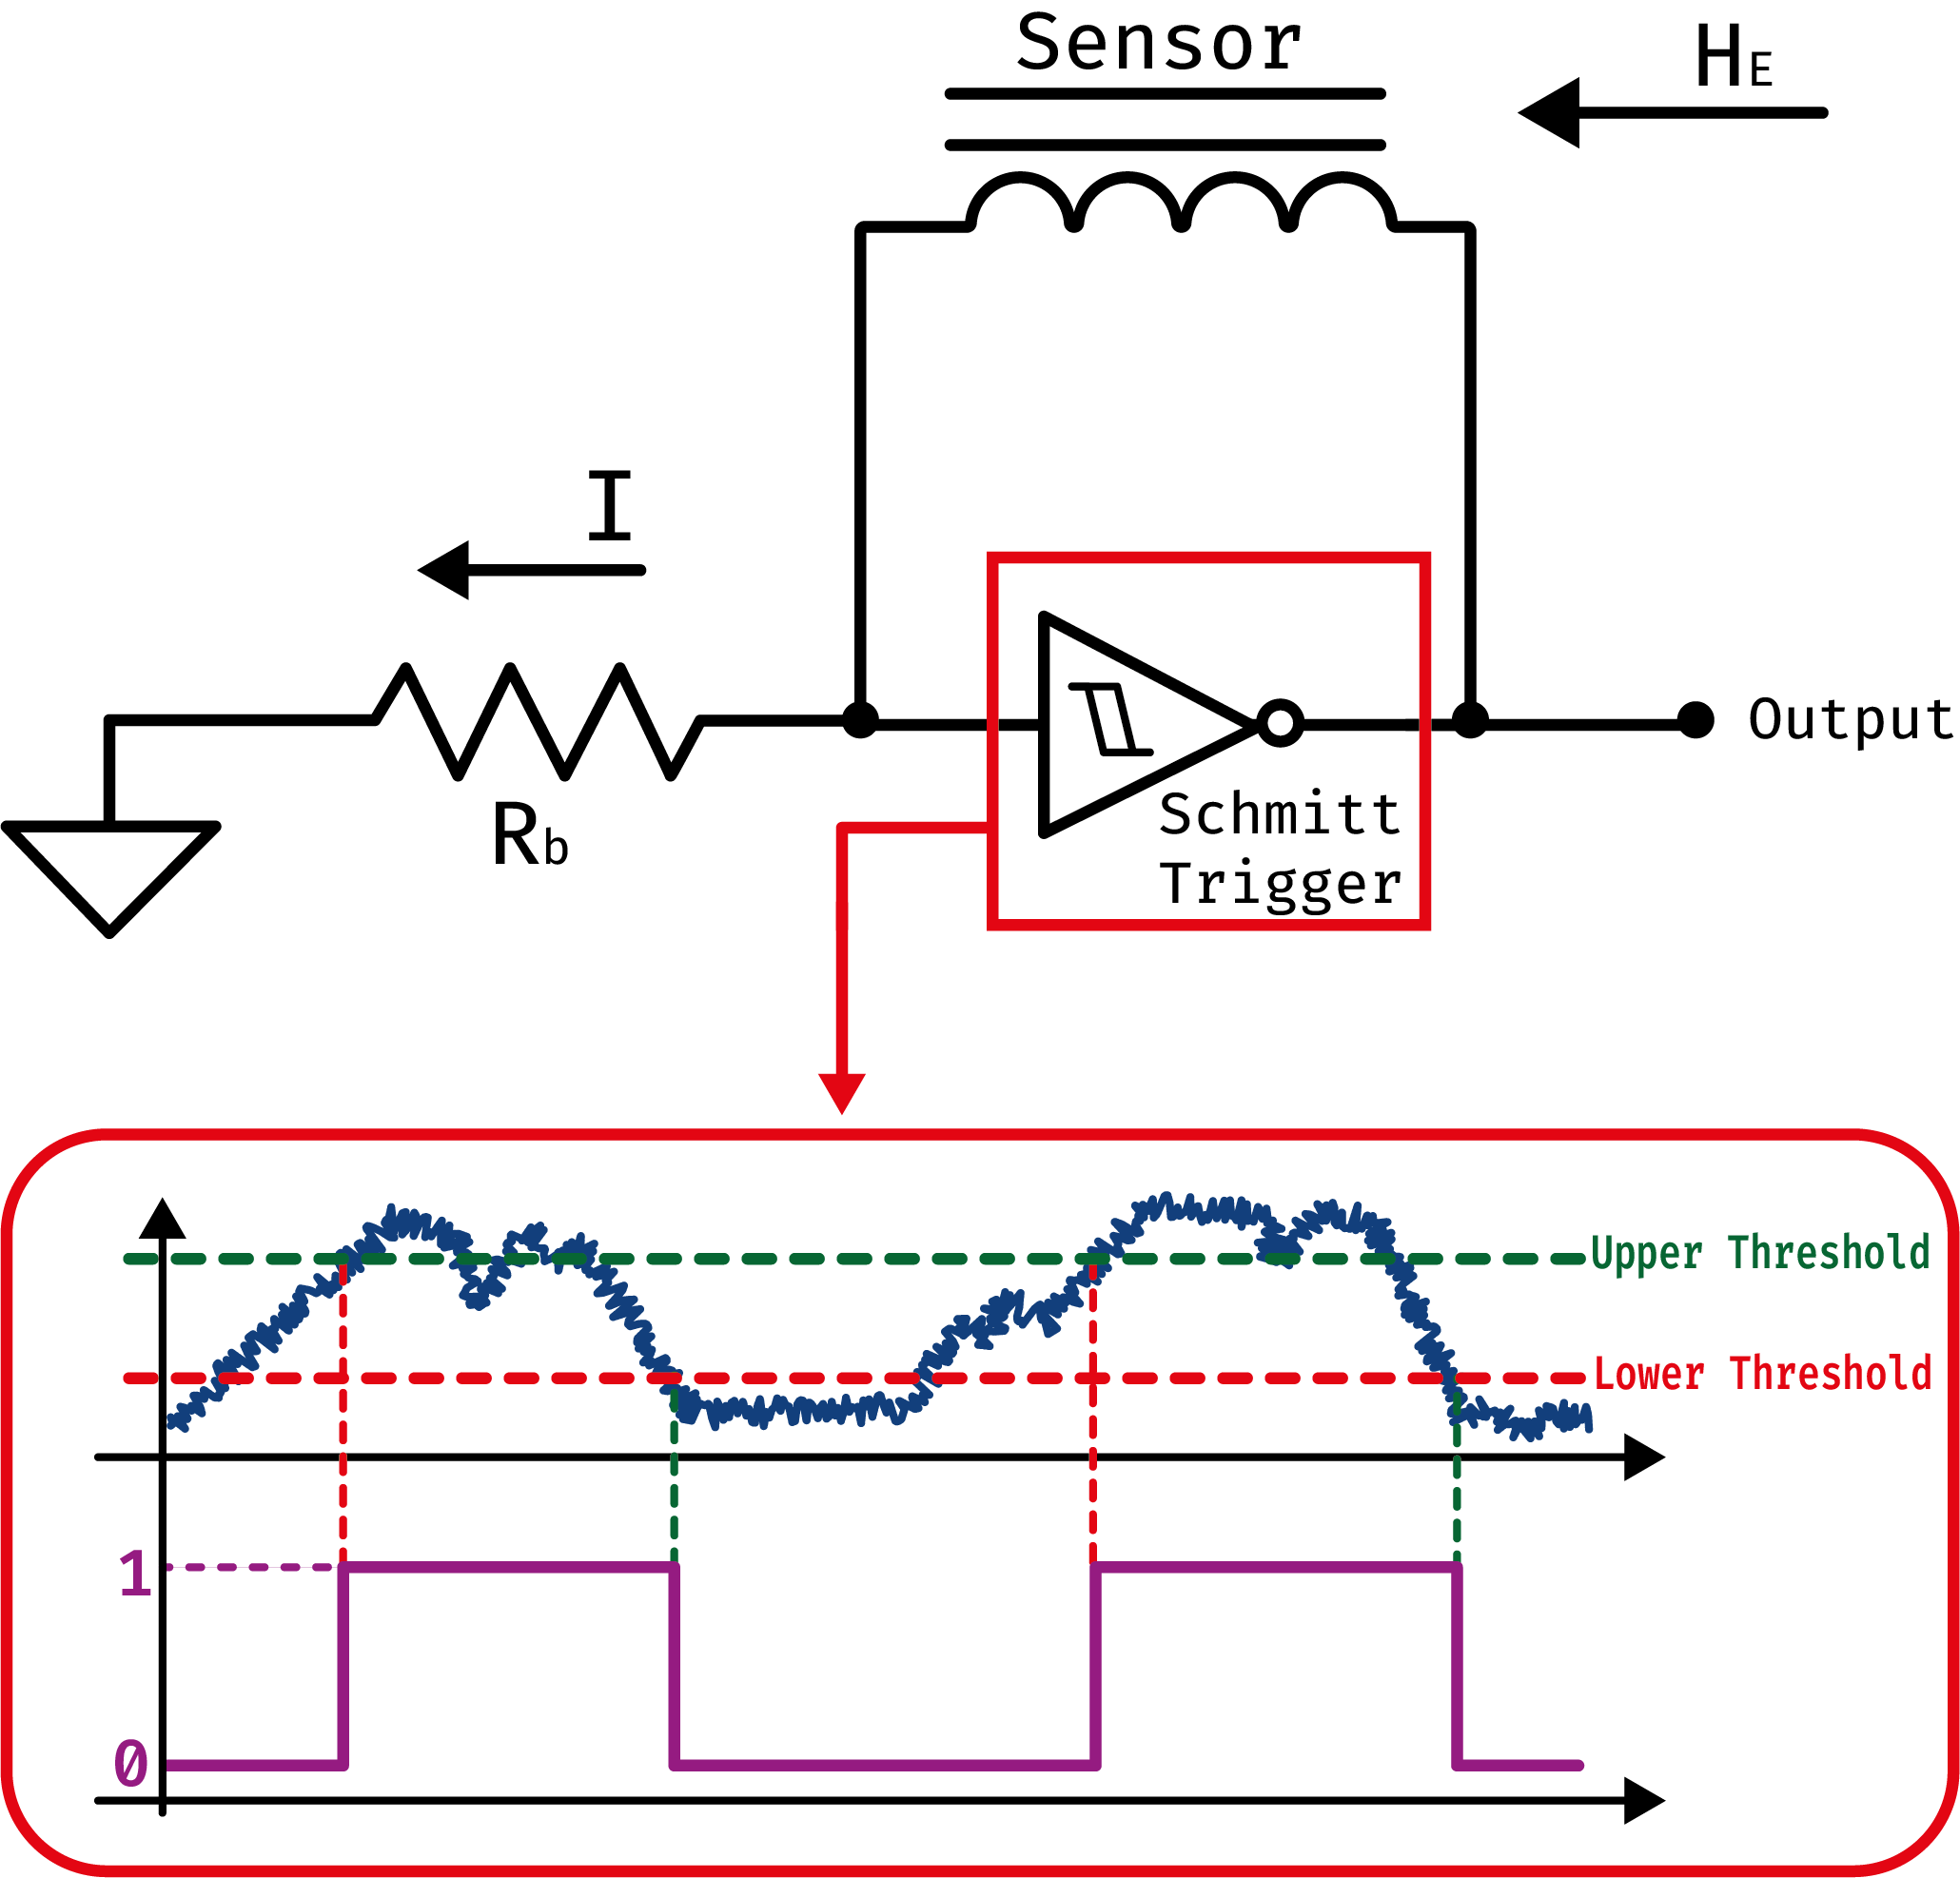
\includegraphics[width=0.9\columnwidth]{assets/Circuit R-L.png}
    \captionof{figure}{En la parte superior de la Figura se presenta el Basic MI Sensing Circuit \citep{leuzinger2010}, compuesto por el sensor inductivo $L$, el inversor Schmitt Trigger y la resistencia $R_B$. El recuadro inferior muestra la relación temporal entre la señal de entrada analógica y la salida digital resultante, donde el trazo azul representa la variación de voltaje en el nodo de entrada del Schmitt Trigger, la línea verde corresponde al umbral superior (Upper Threshold) y la línea roja al umbral inferior (Lower Threshold).}
    \label{fig:circuito-RL}
\end{center}

Añadido a esto, el Schmitt trigger de la \cref{fig:circuito-RL} corresponde a un tipo de entrada lógica que proporciona histéresis o dos niveles de voltaje de threshold diferentes para el edge ascendente y descendente. Es decir, sensa una tensión proporcional a la corriente y conmuta su salida cuando esa tensión cruza un umbral. Para entender mejor esto, se tomará un semiciclo de carga que lleva corriente desde $-I_{th}$ hasta $I_{th}$, con umbrales simétricos $I_{th} = V_{th}/R_b$, por lo que imponiendo estas condiciones en la \cref{eq:3}:
\begin{equation*}
    I_{th} = I_{\infty} + (-I_{th}-I_{\infty})e^{-T/\tau}
\end{equation*}
despejando la exponencial:
\begin{align}
    &e^{-T/\tau}
        = \dfrac{I_{\infty} - I_{th}}{I_{\infty} + I_{th}} \notag \\
    &\Longleftrightarrow\ T
        = \tau \ln\!\left(\dfrac{I_{\infty} + I_{th}}{I_{\infty} - I_{th}}\right) \notag \\
    &\boxed{\;T = \dfrac{L}{R_b}\,
        \ln\!\left(\dfrac{V_S + V_{th}}{V_S - V_{th}}\right)
        }= K\,\dfrac{L}{R_b}\;
    \label{eq:5}
\end{align}

El resultado obtenido en la \cref{eq:5} es que el tiempo de un semiciclo es proporcional a $L$ (y por lo tanto a $\mu(H)$), con un factor $K$ que depende únicamente de la excitación de $V_S$ y de los umbrales $V_{th}$. La condición de oscilación es $V_S > V_{th}$, para que el argumento del logaritmo sea positivo y finito.

Sin embargo, cabe mencionar que hay ciertas cosas que separar de la funcionalidad del Schmitt trigger, ya que este no interviene en la física del campo y las \cref{eq:1,eq:2}, ya que son independientes del trigger. Lo que sí hace este elemento es que sostiene la oscilación, debido a que un circuito $L/R$ por sí solo relaja una única vez hacia $I_{\infty}$ y se detiene. El Schmitt trigger, al tener dos umbrales, al cruzar el alto conmuta e invierte la excitación, la corriente relaja hacia el otro extremo y cruza el umbral bajo, donde vuelve a conmutar, manteniendo una oscilación de relajación permanente. También fija la ventana de medida, donde el intervalo va siempre de un umbral fijo al otro, en el que el tiempo medido es la \cref{eq:5} y no distorsiona la dependencia de $T$ con el campo, solo la escala. Por último, genera las dos polaridades de bias ya que, en cada semiciclo la corriente tiene signo opuesto y esto produce los dos puntos de operación. En resumen, el trigger no cambia lo que se mide, sino que hace posible medirlo, anclando la medida a una ventana temporal definida.

\subsection{Bias en dos polaridades y medida diferencial}
Como se mencionó anteriormente, el oscilador excita el núcleo alterando el signo de la corriente \citep{leuzinger2010,regoli2018}. Según \cref{eq:1}, con una corriente de bias de magnitud característica $I_b$ y $H_b \equiv k_0I_b$, los dos puntos de operación son
\begin{align}
    \text{bias directo (forward): }& H_+ = +H_b + H_E \\
    \text{bias inverso (reverse): }& H_- = -H_b + H_E
\end{align}
donde el bias sitúa estos dos puntos sobre los flancos inclinados de la curva $\mu_{inc}(H)$, que tiene forma de campana, como se muestra en la \cref{fig:sensor_no_he}. Esta curva es la pendiente  $dB/dH$ de la curva B-H de la \cref{fig:curva-bh}, y su forma es la que se reporta en \citet{leuzinger2010}, ya que $L = G\mu_{inc}$. La \cref{fig:sensor_operation} detalla el mecanismo, donde en cada polaridad la corriente no se queda en un punto, sino que barre una ventana de excursión entre los umbrales de carga $H_L$ y $H_H$ (que son los umbrales del Schmitt trigger en unidades de campo), situada por el bias $H_b$ sobre uno de los flancos. Las trazas inferiores son las curvas de carga y descarga, cuya duración es $\tau_P$ (bias positivo, banda verde) y $\tau_N$ (bias negativo, banda roja).

Usando \cref{eq:5,eq:2} con $H = \pm H_b + H_E$, el tiempo medio en cada polaridad sobre un número fijo de ciclos $N_C$ es $t_{\pm} \propto \mu_{inc}(\pm H_b + H_E)$, por ende:
\begin{align}
    t_{\pm} &= N_c\ T_{\pm} \notag\\
            &= N_C K\dfrac{L}{R_b} \notag\\
            &= \dfrac{KGN_C}{R_b}\mu_{inc}(\pm H_b + H_E) \quad ; C_0 =\dfrac{KGN_C}{R_b} \notag\\
    &\Longrightarrow t_+ = C_0\mu_{inc}(+H_b+H_E)\\
    &\Longrightarrow t_- = C_0\mu_{inc}(-H_b + H_E)       
\end{align}

Sin campo externo ($H_E = 0$), como $\mu_{inc}$ es par, entonces $\mu_{inc}(H_b) = \mu_{inc}(-H_b)$, de modo que $t_+ = t_-$ y la diferencia se anula, generando el cero natural del instrumento.
\begin{align}
    t_+ = C_0 \mu_{inc}(H_b) &= C_0 \mu_{inc}(-H_b) = t_-\\
    \Longrightarrow \Delta t & \equiv t_+ - t_- = 0
\end{align}
Con campo externo ($H_E \neq 0$) y suponiendo que $H_E \ll H_b$, se puede hacer una expansión de Taylor de $\mu_{inc}$ alrededor de $\pm H_b$ a primer orden, teniendo:
\begin{align*}
    \mu_{inc}(+H_b + H_E) &\approx \mu_{inc}(H_b) + \mu_{inc}'(H_b)H_E\\
    \mu_{inc}(-H_b + H_E) &\approx \mu_{inc}(-H_b) + \mu_{inc}'(-H_b)H_E
\end{align*}
restando estos dos resultados y recordando que $\mu_{inc}$ es par ($\mu_{inc}(H_b) = \mu_{inc}(-H_b)$) y su derivada $\mu_{inc}'$ es impar ($\mu_{inc}'(-H_b) = -\mu_{inc}'(H_b)$), se obtiene que:

\begin{align}
    \Delta t &= t_+ - t_- \notag \\
              &\approx C_0\left[\mu_{inc}'(H_b)-\mu_{inc}'(-H_b)\right]H_E \notag \\
              &= 2C_0\mu_{inc}'(H_b)H_E \notag \\
    \Delta t &= \dfrac{2KGN_C}{R_b} \mu_{inc}'(H_b)H_E \propto H_E
    \label{eq:6}
\end{align}

por ende, la diferencia de tiempos entre las dos polaridades es lineal en el campo externo $H_E$ por medio de una constante de escala, siendo este el principio de medida del sensor. La sensibilidad es proporcional a $\mu_{inc}'(H_b) = d^2B/dH^2|_{H_b}$, es decir, a la curvatura de la curva B-H en el punto del bias. 

\begin{center}
    \captionsetup{type=figure}% establece el tipo (necesario para subcaptions fuera de un float)
    \subcaptionbox{Sin campo externo ($H_E = 0$)\label{fig:sensor_no_he}}
        {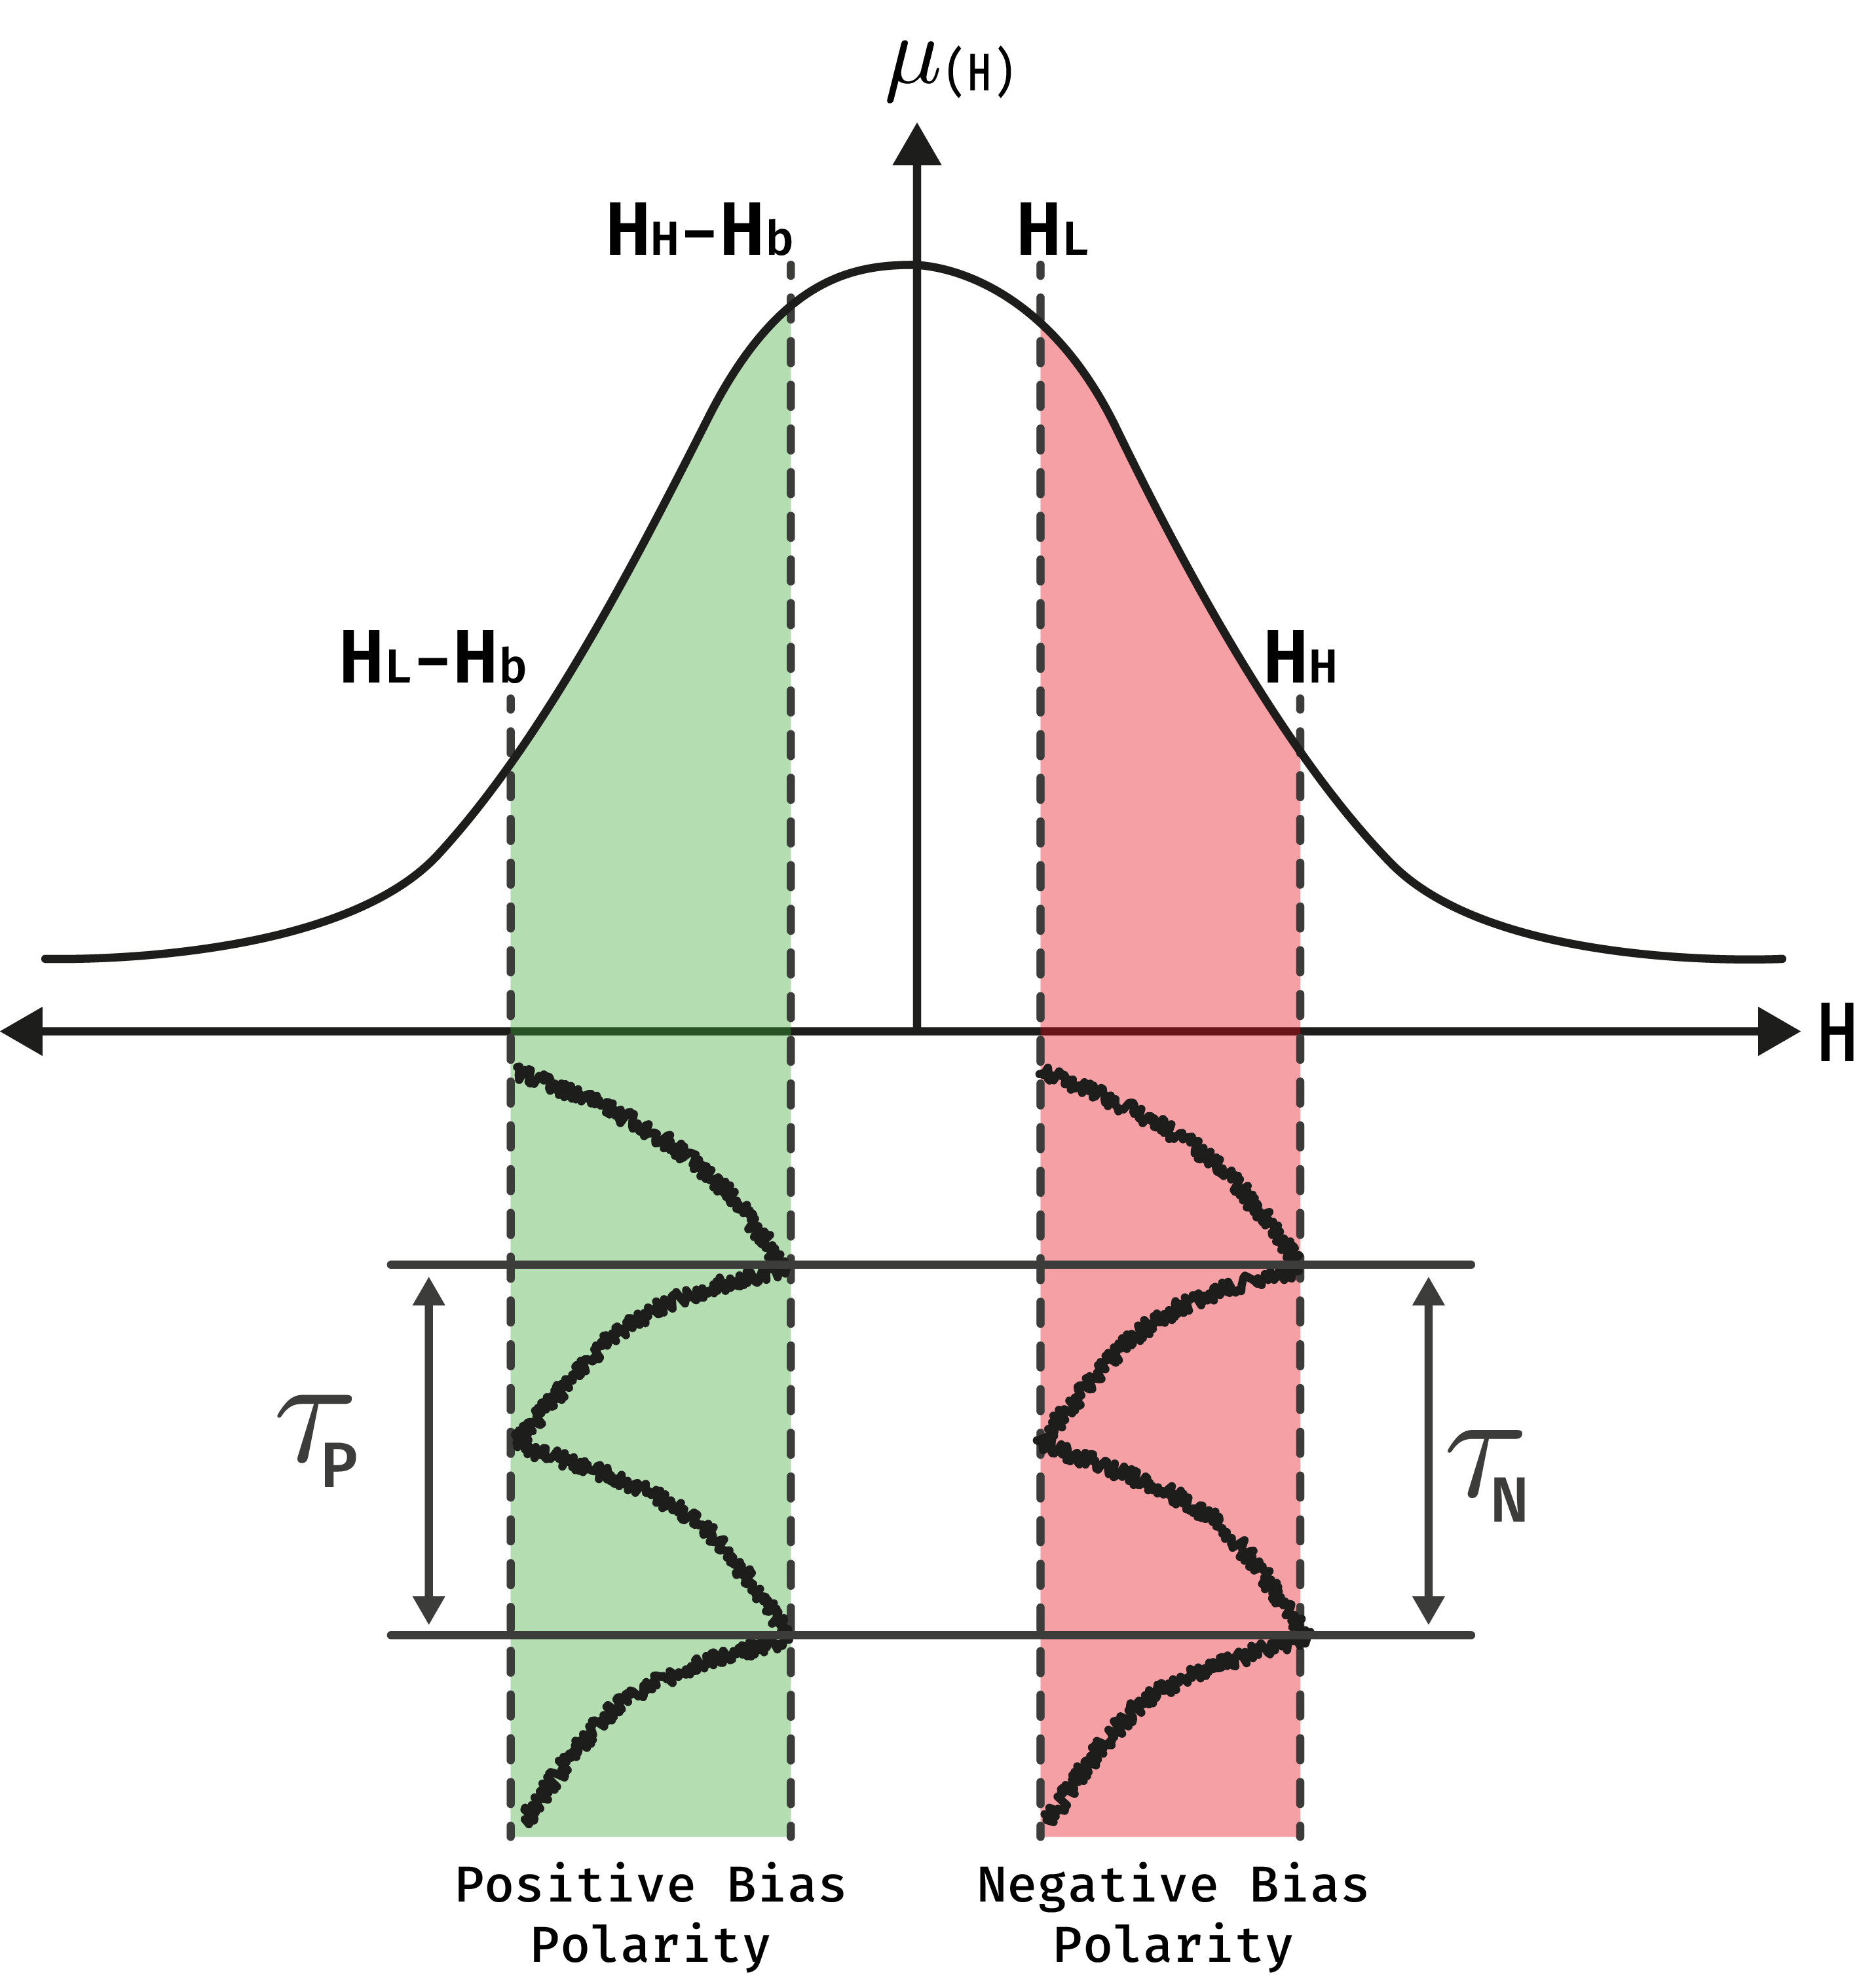
\includegraphics[width=0.9\columnwidth]{assets/Sensor_operation_NO_HE.png}}%
    \\[30pt]
    \subcaptionbox{Con campo externo ($H_E \neq 0$)\label{fig:sensor_si_he}}
        {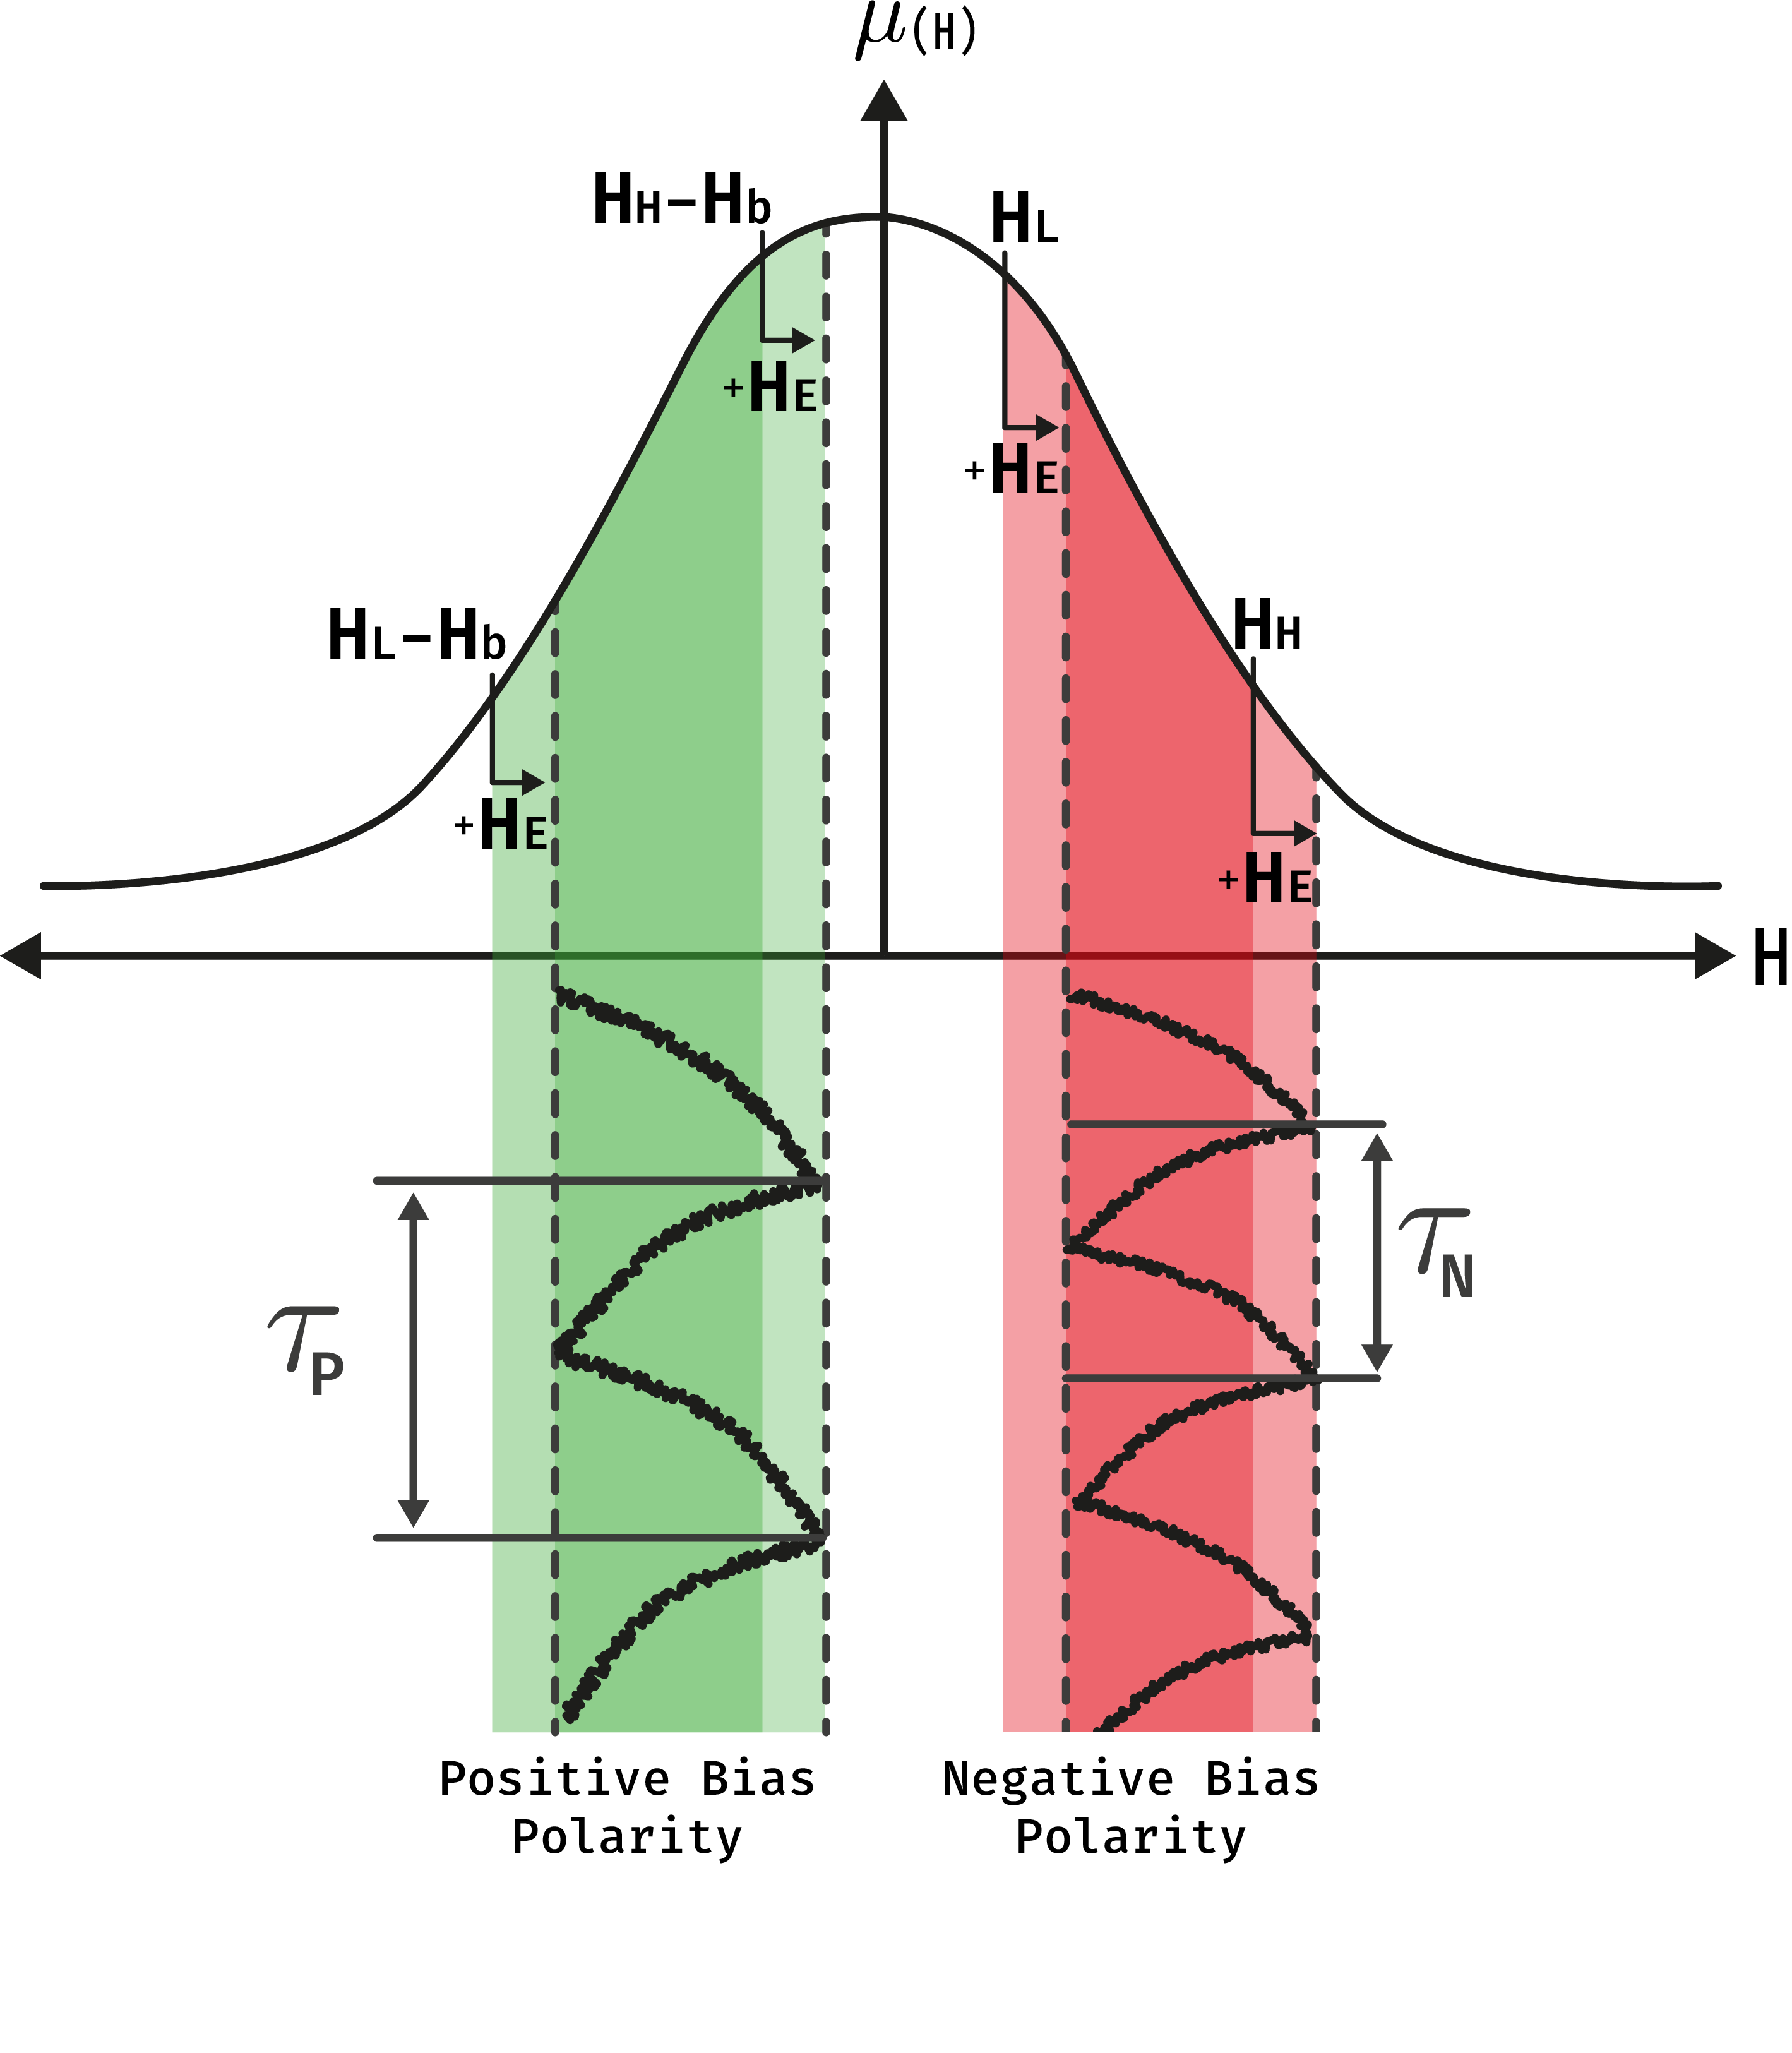
\includegraphics[width=0.9\columnwidth]{assets/Sensor_operation_SI_HE.png}}

    \captionof{figure}{Operación del bias en las dos polaridades sobre la curva de permeabilidad $\mu_{inc}(H)$. Cada polaridad barre una ventana de excursión delimitada por los umbrales de carga (lineas discontinuas), donde $H_L$ y $H_H$ para la polaridad negativa (banda roja) y los mismos desplazados por el bias, $H_L - H_b$ y $H_H - H_b$, para la positiva (banda verde). Las trazas inferiores son la curva de carga y descarga, con duración $\tau_P$ y $\tau_N$. (a) Sin campo externo, las ventanas quedan simétricas sobre la campana y $\tau_P = \tau_N$, donde la diferencia se anula. (b) Un campo externo $H_E$ desplaza ambas ventanas en el mismo sentido (bandas claras y flecha $+H_E$), donde al estar sobre flancos de pendiente opuesta, la permeabilidad promedio sube en una polaridad y baja en la otra, de modo que $\tau_P \neq \tau_N$ y $\tau_P - \tau_N \propto H_E$. Esta es una imagen adaptada del esquema de \citet{regoli2018} y de \citet{leuzinger2010}.}
    \label{fig:sensor_operation}
\end{center}

Este modelo diferencial coincide con la operación que describe el manual de RM3100 \citep{pni_manual}. Para medir, el ASIC mantiene un extremo de la bobina a tierra y excita el otro alternando corriente positiva y negativa, contando un número fijo de oscilaciones del circuito en cada polaridad y mide su duración con el reloj interno. Como el campo inducido por el circuito tiene ``la misma magnitud y dirección opuesta para las dos polaridades del bias'', el manual concluye que el campo local es proporcional a la diferencia de tiempos entre las direcciones directa e inversa, ya que la diferencia de cuentas de reloj que entrega el ASIC es directamente proporcional al campo \citep{pni_manual}. Esto es lo que se muestra en la \cref{eq:6}, donde el campo inducido de igual magnitud y signo opuesto es el $\pm H_b$ de \cref{eq:1}, y la salida proporcional a la diferencia es $\Delta t \propto H_E$.


\section{Arquitectura del sensor}
Como se mencionó en el resumen, el sensor RM3100 es un conjunto formado por tres bobinas sensoras y un circuito integrado de aplicación específica (ASIC) que las controla \citep{pni_manual}. La \cref{fig:diagrama_bloques} muestra el diagrama de bloques, donde el ASIC MagI2C ocupa el centro, ya que enlaza el microcontrolador a utilizar por medio de SPI o I$^2$C con las tres bobinas sensoras (una por cada eje $X, Y, Z$). Cada bobina, junto con un resistor de bias externo $R_b$ y el comparador interno del ASIC, forman un oscilador de relajación L/R independiente. Un resistor externo $R_{EXT}$ fija el reloj de alta velocidad con el que el ASIC mide los tiempos de oscilación. 

\begin{center}
    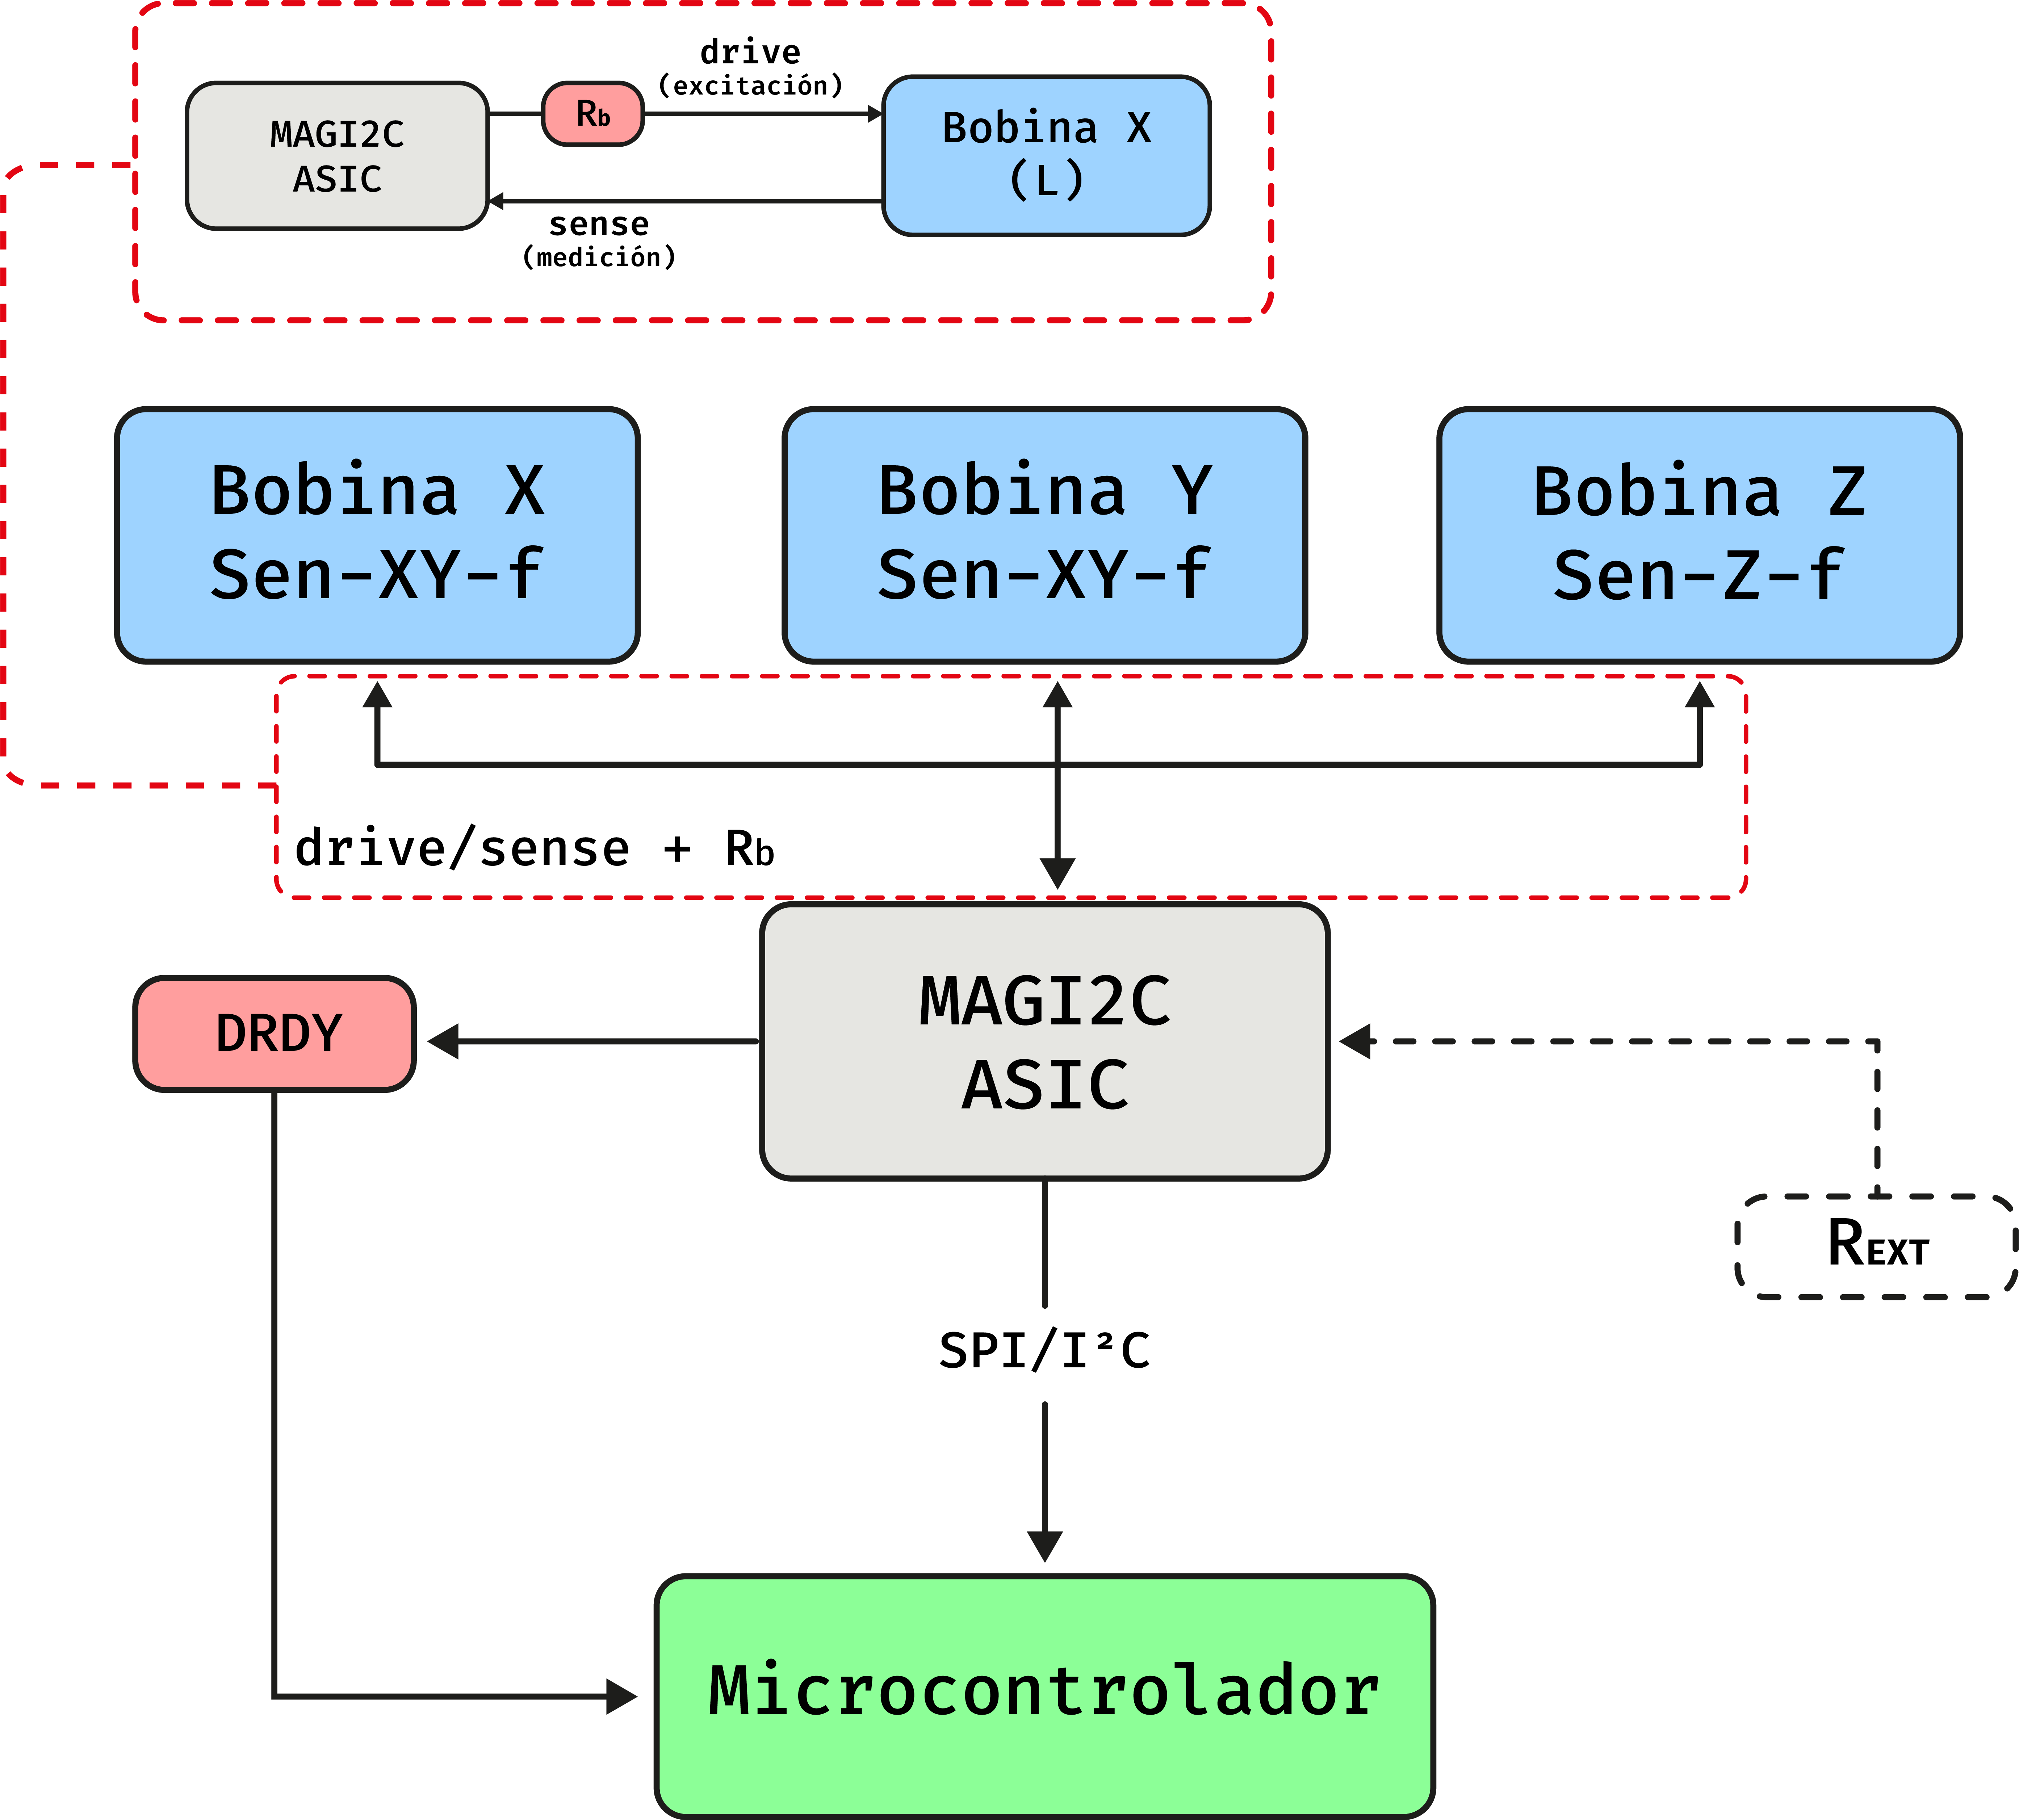
\includegraphics[width=0.9\columnwidth]{assets/Diagrama-bloques-RM3100.png}
    \captionof{figure}{Diagrama de bloques del RM3100. El ASIC MagI2C enlaza el microcontrolador (por SPI o I$^2$C) con las tres bobinas del sensor. Cada eje forma un oscilador L/R con su bobina, el resistor de bias $R_b$ y la electrónica interna del ASIC. $R_{EXT}$ fija el reloj de medida y la línea DRDY avisa cuando hay un dato disponible. Dentro del cuadro en rojo se encuentra el desglose de la conexión de una bobina y el ASIC. La rama de drive (pines XDRVP/XDRVN; YDRVP/YDRVN; ZDRVP/ZDRVN) inyecta la corriente por el resistor de bias externo $R_b$, mientras que la rama sense (pines XINP/XINN; YINP/YINN; ZINP/ZINN) lleva el nodo de la bobina al comparador interno. El ASIC alterna cuál extremo se excita y cuál se aterriza, generando las dos polaridades de bias.}
    \label{fig:diagrama_bloques}
\end{center}

Como se mencionó anteriormente, los principales componentes del sensor RM3100 son los que se verán a continuación; sin embargo, cabe mencionar que \citet{pni_manual} entrega ciertos valores de referencia para el resto de componentes, como se ve en la \cref{tab:electricos}.

\textbf{Bobina sensora:} Cada bobina es un solenoide de geometría alargada devanado sobre un núcleo de alta permeabilidad, y actúa como elemento inductivo del oscilador. La Sen-XY-f es insensible a la ubicación de su marca de polaridad, mientras que en la Sen-Z-f esa marca sí es necesaria para la orientación. La \cref{fig:view-sensor} muestra cómo son estos sensores en la realidad.

\textbf{ASIC Mag I2C:} Aloja las compuertas digitales y el comparador que, con la bobina y $R_b$, cierran el oscilador; el reloj de alta velocidad que mide los tiempos; y la lógica del cycle count junto con las interfaces SPI e I$^2$C. Esto se entrega en encapsulado MLF de 28 pines y se clasifica como MSL 3. Al trabajar en el dominio de frecuencia y entregar un valor digital, elimina el conversor A/D y el amplificador.

\begin{center}
    \captionof{table}{Parámetros eléctricos típicos ($V_{\mathrm{DD}}=3.0$~V, temperatura ambiente) \citep{pni_manual}.}
    \label{tab:electricos}
    \small
    \begin{tabular}{@{}l c@{}}
        \hline
        Parámetro & Valor típico \\
        \hline
        Resistor de bias, $R_b$            & $121\ \Omega$ \\
        Resistor de reloj, $R_{\mathrm{EXT}}$ & $33\ \mathrm{k}\Omega$ \\
        Frecuencia de oscilación, $f_{\mathrm{osc}}$ & $180\ \mathrm{kHz}$ \\
        Inductancia de bobina, $L$         & $500$--$600\ \mu$H \\
        Resistencia de bobina, $R_{\mathrm{coil}}$ & $30$--$45\ \Omega$ \\
        Alimentación, $V_{\mathrm{DD}}$    & $2.0$--$3.6$~V \\
        Temperatura de operación           & $-40$ a $+85\ ^\circ$C \\
        \hline
    \end{tabular}
\end{center}

\begin{center}
    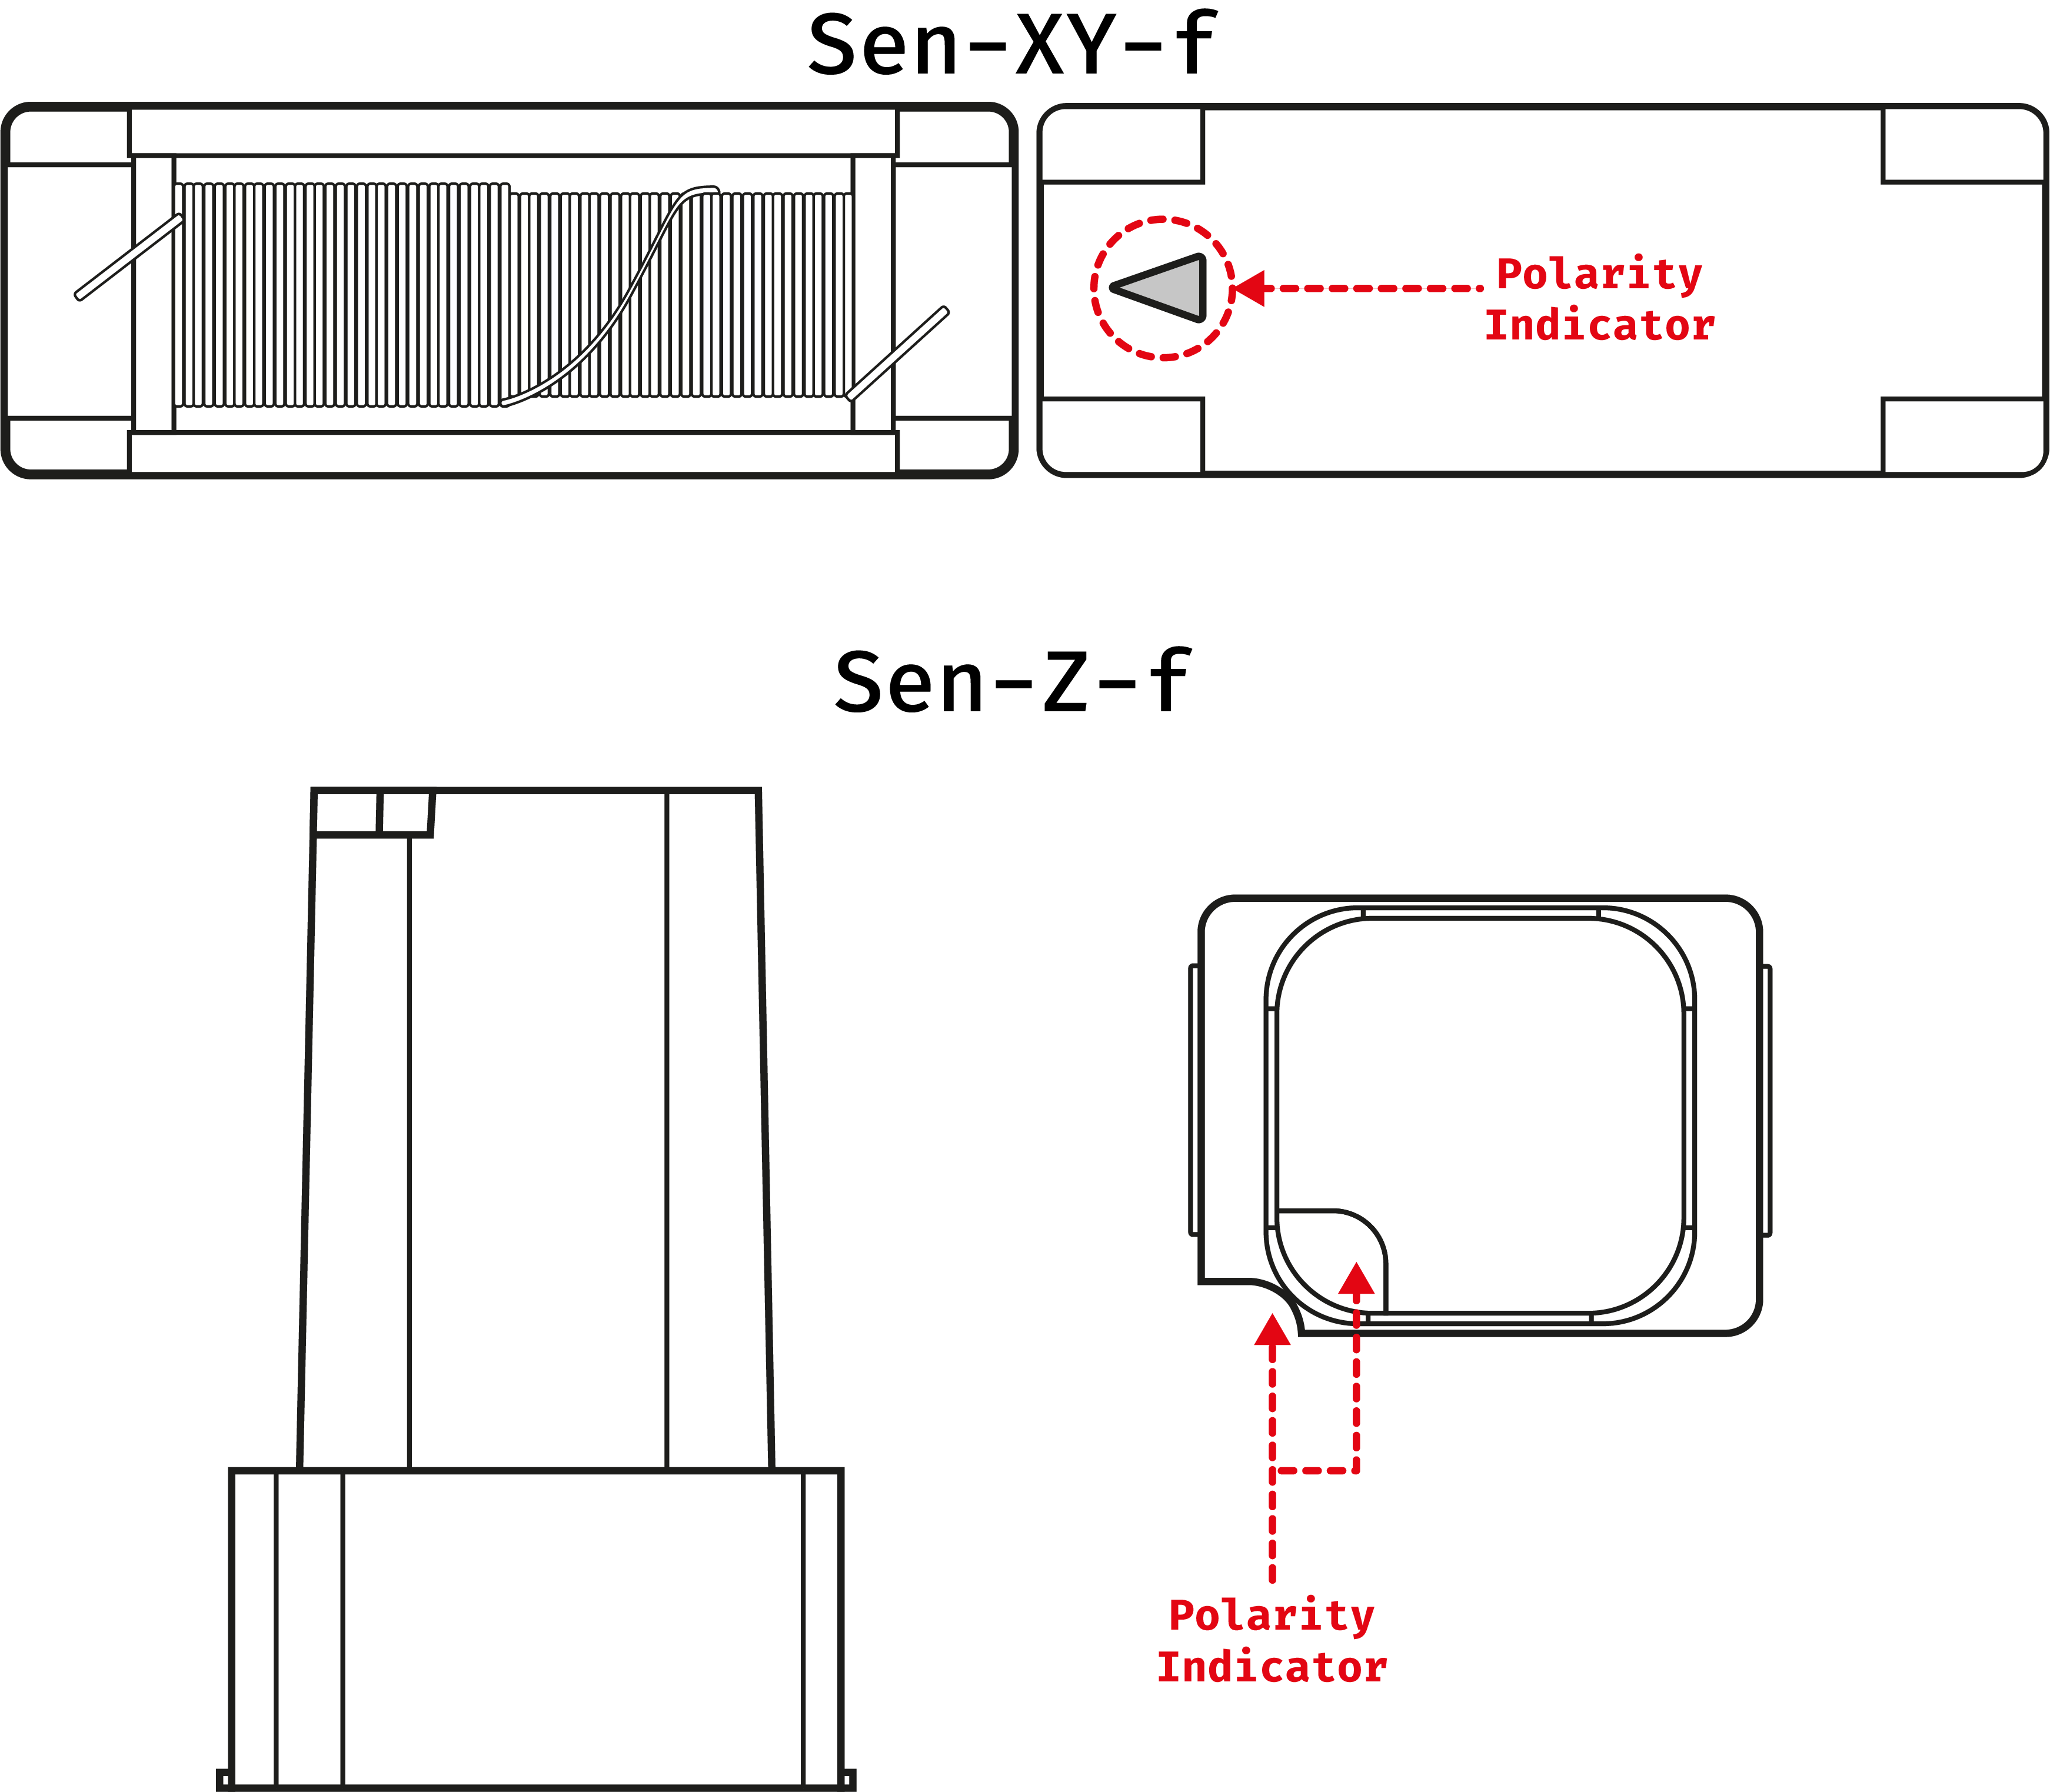
\includegraphics[width=0.9\columnwidth]{assets/View-Sensor-inductor.png}
    \captionof{figure}{Diagrama basado en \citet{pni_manual} que tiene la estructura del sensor Sen-XY-f en la parte de arriba, además de la indicación de polarización y el Sen-Z-f, que se encuentra en la parte de abajo y muestra su estructura.}
    \label{fig:view-sensor}
\end{center}

Las tres bobinas se disponen ortogonalmente en un marco NED (north-east-down), donde cada canal representa un eje cartesiano. La flecha impresa en el módulo indica la línea de mira y es paralela a cada eje. Por ser un instrumento vectorial, la ortogonalidad y el alineamiento de las bobinas condicionan la exactitud direccional.

El ASIC separa los dominios analógico y digital. AVDD y DVDD alimentan las secciones analógica y digital, con AVSS y DVSS como sus retornos; DVDD debe estar presente siempre que lo esté AVDD, y AVDD puede apagarse entre medidas para ahorrar energía sin perder el contenido de los registros, que se retiene mientras DVDD siga alimentado \citep{pni_manual}. Las señales de control principales son: $R_{\mathrm{EXT}}$ (fija el reloj de alta velocidad), DRDY (se pone en alto cuando hay una medida disponible), I2CEN (selecciona interfaz: alto para I\textsuperscript{2}C, bajo para SPI) y los pines de drive y sense hacia cada bobina. El dispositivo arranca en modo de reposo (idle) y regresa a él automáticamente cuando no mide ni intercambia datos, con un consumo de reposo del orden de $1\ \mu$A.

El MagI2C ofrece dos interfaces seleccionables por hardware mediante el pin I2CEN, lo que da flexibilidad de integración \citep{pni_manual}. En SPI actúa como esclavo con las líneas SCLK, MOSI, MISO y SSN, con reloj de $1$~MHz o menos. En I\textsuperscript{2}C usa SDA y SCL con una dirección de $7$ bits cuyos cinco bits altos son fijos (0b01000) y los dos bajos se configuran por pines, lo que permite cuatro direcciones distintas en el mismo bus. Los mismos cuatro pines de comunicación cambian de función según la interfaz elegida, como resume la \cref{tab:pines}.
 
\begin{center}
    \captionof{table}{Pines del MagI2C que intervienen en las interfaces SPI e I\textsuperscript{2}C \citep{pni_manual}. Los cuatro primeros son de doble función.}
    \label{tab:pines}
    \footnotesize
    \begin{tabular}{@{}c c c p{3.9cm}@{}}
        \hline
        Pin & SPI & I\textsuperscript{2}C & Función \\
        \hline
        1  & MOSI & SDA & Datos: host$\rightarrow$ASIC en SPI; línea bidireccional (SDA) en I\textsuperscript{2}C \\
        27 & SCLK & SCL & Reloj serie generado por el host ($\leq 1$~MHz) \\
        28 & MISO & SA1 & Datos ASIC$\rightarrow$host en SPI; bit 1 de la dirección de esclavo en I\textsuperscript{2}C \\
        3  & SSN  & SA0 & Selección de esclavo (activo en bajo) en SPI; bit 0 de la dirección en I\textsuperscript{2}C \\
        22 & \multicolumn{2}{c}{I2CEN} & Selecciona la interfaz: alto $=$ I\textsuperscript{2}C, bajo $=$ SPI \\
        23 & \multicolumn{2}{c}{DRDY} & Línea de estado: se pone en alto cuando hay una medida disponible \\
        \hline
    \end{tabular}
\end{center}
 
El pin I2CEN debe fijarse en alto o bajo según la interfaz. La línea DRDY es opcional: el mismo aviso de dato disponible puede obtenerse leyendo el registro STATUS, o, en SPI con CPOL$=$CPHA$=$1, observando la línea MISO \citep{pni_manual}. En ambas interfaces la comunicación es por registros; el mapa de registros y las secuencias de operación se detallan en el capítulo de interfaces y operación.

El conjunto ocupa un área del orden de $2.54\times2.54\ \mathrm{cm}^2$ con una masa menor a $3$~g \citep{regoli2018}. Para preservar el desempeño, el manual recomienda situar las bobinas lo más cerca posible entre sí (para reducir el efecto de gradientes del campo), mantener el MagI2C a menos de $10$~cm de las bobinas con las trazas de cada par juntas (para reducir acoplamientos) y alejar los capacitores, en especial los de tantalio, de las bobinas \citep{pni_manual}. Las bobinas requieren pastas y procesos de soldadura libres de haluros. Estas reglas de integración son parte del diseño del sistema; la interferencia magnética externa y la estabilización térmica se tratan en el capítulo de consideraciones prácticas.


\section{Modelo de medición}

En la sección anterior, se estableció que la diferencia de tiempo entre las dos polaridades de bias es lineal en el campo externo $\Delta t = t_+ - t_- \propto H_E$ (\cref{eq:6}). El modelo de medición describe cómo esa magnitud temporal se convierte en un número digital con signo y, finalmente en un valor de campo por eje en unidades de $\mu T$. 

El ASIC no cronometra $\Delta t$ de forma analógica. Conviene distinguir dos frecuencias: la de oscilación propia del circuito $L/R, \ f_{osc} \approx 180\ kHz$ (fijada por el sensor), y la del reloj interno de alta velocidad, fijada por el resistor externo $R_{EXT} = 33\ k\Omega$. Para medir, el ASIC excita cada bobina durante un número fijo de ciclos $N_C$ (cycle count) en cada polaridad y cuenta pulsos de $f_{clk}$ para cronometrar esa ventada. La salida por eje es el count difference
\begin{equation*}
    \Delta C = f_{clk} \Delta t \propto H_E
\end{equation*}

Esa diferencia, con signo, se almacena en los registros de resultados como un entero de 24 bits (3 bytes) en complemento a dos, con rango $-8388608$ a $8388607$ \citep{pni_manual}. Se denota $M_i \ [LSB]$ a la cuenta cruda del eje $i$, donde $LSB$ es Least Significant Bit.

Esta constante de proporcionalidad entre $M_i$ y el campo es la ganancia, en $LSB/\mu T$, y depende del cycle count, , a más ciclos, más cuentas por unidad de campo. El manual tabula la ganancia para $N_C = \{50, 100, 200\}$ como $gain = \{20, 38, 75\}\ LSB/\mu T$ \citep{pni_manual}. Por este motivo, al hacer un ajuste lineal de mínimos cuadrados sobre estos tres puntos, se llega a la siguiente ecuación

\begin{equation}
    gain(N_C) = 0.3671N_C + 1.5000 \ [LSB/\mu T]
    \label{eq:8}
\end{equation}

de acuerdo a la \cref{eq:8} y válida en el rango útil $(\sim 30\text{ a } 400)$. El término independiente sirve de ajuste sobre los tres puntos y no sería un offset físico. Con esto, la dependencia esperada es que $\text{gain } \propto N_C$, obteniendo que la cuenta cruda de cada eje, la magnitud del capo por eje y el modulo son:

\begin{equation}
    B_i = \dfrac{M_i}{gain}, \qquad B = \sqrt{B_x^2 + B_y^2 + B_z^2}
    \label{eq:9}
\end{equation}

\begin{center}
    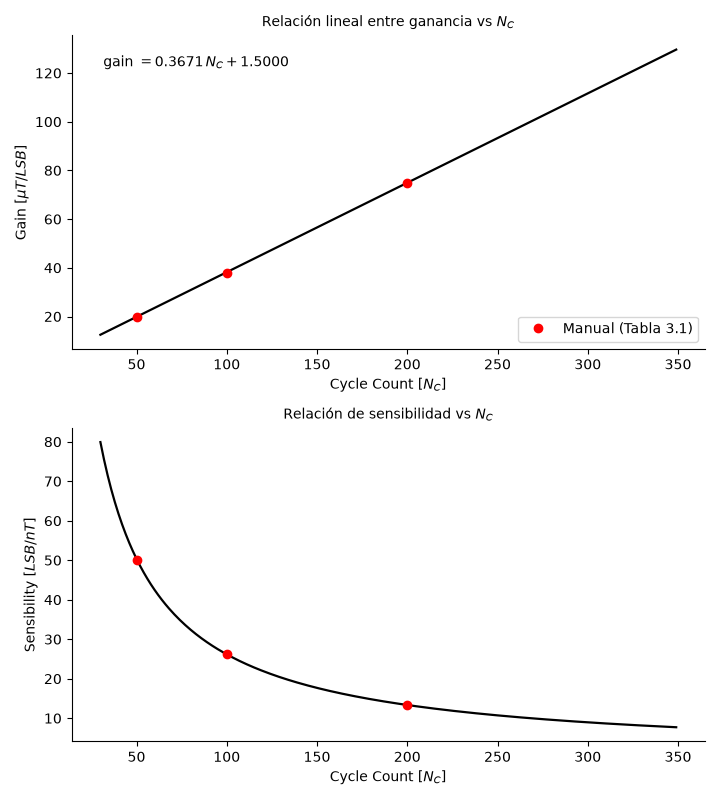
\includegraphics[width=1\columnwidth]{assets/CycleCount_Gain_Sensibility.png}
    \captionof{figure}{La primera imagen es la Ganancia vs el Cycle counto, donde los tres valores en rojo son los valores dados por el manual y se encuentran en la recta obtenida en la \cref{eq:8}. El segundo gráfico es la sensibilidad obtenidoa como $q=1/\text{gain}$, donde esta curva reproduce los valores de sensibilidad del manual, lo que valida el modelo. Por lo tanto, subir el $N_C$ aumenta la ganancia y reduce el paso de cuantización (mejor resolución) a costa del tiempo de adquisición.}
    \label{fig:gain_cycle_sensibility}
\end{center}

como se menciona en la \cref{fig:gain_cycle_sensibility}, la resolución del campo es dada por
\begin{equation}
    q(N_C) = \dfrac{1}{gain(N_C)} \ [\mu T /LSB]
    \label{eq:10}
\end{equation}

con la \cref{eq:10}, $q = \{50, 26, 13\}\ nT$ para $N_C=\{50, 100, 200\}$, lo que coincide con la sensibilidad entregada por el manual \citep{pni_manual} (\cref{tab:gain}). El ruido, en cambio, se obtiene de forma distinta a la resolución. Esta ultima se calcula como $q=1/gain$ y es determinista, es decir, se deduce de la ganancia y es el paso de cuantización (cuántos $nT$ vale una cuenta). El ruido es una cantidad estadística, donde la dispersión (RMS) de medir repetidamente un mismo campo constante, originada por el ruido térmico y electrónico del ASIC y por una componente $1/f$. Este valor no se deriva de la ganancia, sino que se caracteriza experimentalmente, por eso los valor del ruido de la \cref{tab:gain} se toma directamente del manual \citep{pni_manual}, y no de una fórmula. En el dominio espectral, este ruido tiene un piso de $4\ pT/\sqrt{Hz}$ a $1\ Hz$ \citep{regoli2018}, siendo la densidad que se relaciona con el ruido RMS temporal integrándola sobre el ancho de banda de medida.

Sobre el ruido sí actua una relación cuantitativa, siendo el promedio o oversampling. Si se promedian $N$ muestras con ruido aleatorio e independiente, las varianzas se suman y la desviación estándar del promedio decae como

\begin{equation}
    \sigma_N = \dfrac{\sigma_1}{\sqrt{N}}
        \label{eq:11}
\end{equation}

con $\sigma_1$ siendo el ruido de una sola muestra. Los datos de \citet{regoli2018} siguen esta ley de forma aproximada: promediar $4$ muestras baja el ruido a $<5$~nT, $20$ muestras a $\sim\!2.7$~nT y $40$ muestras (cadencia $1$~s) a $\sim\!2.2$~nT. Este ajuste no es exacto, porque la componente $1/f$ promedia peor que el ruido blanco, de modo que la \cref{eq:11} entrega una cota optimista. Este mismo mecanismo explica porqué el ruido de la \cref{tab:gain} baja al subir $N_C$. Un cycle count mayor integra sobre más ciclos de oscilación en cada lectura (un promedio interno equivale). También se puede promediar en el espacio, ya que \citet{regoli2018} muestra que cuatro RM3100 mejora la resolución por $\sqrt{N}$ sin bajar la frecuencia de muestreo.

El rango de medición es $\pm\!800\ \mu T$, definido como la región monótona de la curva de salida. Esta puede extenderse usando un $R_b$ distinto al que dice el manual.

\begin{center}
    \captionof{table}{Desempeño en función del cycle count
    (Tabla 3-1 del manual, $V_{\mathrm{DD}}=3.0$~V, $R_b=121\ \Omega$, $R_{\mathrm{EXT}}=33$~k$\Omega$, a temperatura ambiente) \citep{pni_manual}. La sensibilidad derivada de la ganancia ($=1/\mathrm{gain}$) reproduce lafila de sensibilidad del manual.}
    \label{tab:gain}
    \small
    \setlength{\tabcolsep}{4pt}
    \begin{tabular}{@{}lccc@{}}
        \hline
        Par\'ametro & \multicolumn{3}{c}{Cycle count $N_C$} \\
                    & 50 & 100 & 200 \\
        \hline
        Ganancia [LSB/$\mu$T]              & 20   & 38  & 75  \\
        Sensibilidad [nT]                  & 50   & 26  & 13  \\
        Ruido [nT]                         & 30   & 20  & 15  \\
        Repetibilidad sobre $200\,\mu$T [nT] & 15 & 8   & 8   \\
        Tasa máx.\ 1 eje [Hz]            & 1600 & 850 & 440 \\
        Tasa máx.\ 3 ejes ($\div3$) [Hz] & 533 & 283 & 147 \\
        Corriente 1 eje a 24 Hz [$\mu$A]    & 70   & 135 & 260 \\
        \hline
    \end{tabular}
\end{center}

La \cref{eq:9} supone un cero ideal y ejes ortonormales. Para medida absoluta hay que descontar el offset de cada eje y corregir la escala y no ortogonalidad
\begin{equation}
    \mathbf{B} = \mathbf{S}(\mathbf{M}-\mathbf{M}_0)
    \label{eq:12}
\end{equation}
con $\mathbf{M} = (M_x, M_y, M_z)^T$ las raw count, $\mathbf{M}_0$ el vector de offset y $\mathbf{S}$ una matríz de $3\times3$ que agrupa la ganancia por eje, la correción de escala relativa y la de no ortogonalidad. En el caso ideal, $\mathbf{S} = diag(1/gain)$ y se recupera la \cref{eq:9}. La determinación de $\mathbf{M}_0$  y $\mathbf{S}$ (ajuste de elipsoide sobre rotaciones en campo constante) queda fuera de alcance de este modelo y se puede abordar más adelante.

\section{Modelo de operación}
El modelo de operación describe cómo el host (ej: microcontrolador) configura y comanda el ASIC MagI2C para obtener cada medida. El MagI2C no mide por iniciativa propia, debido a que parte del reposo (Idle Mode) y solo mide cuando el host escribe en sus registros. Esta operación completa se reduce en cuatro funciones \citep{pni_manual}:
\begin{enumerate}
    \item Fijar los registros de cycle count, de lo contrario se utiliza el valor por defecto.
    \item Iniciar una medición única (POLL) o continua (CMM).
    \item Confirmar que hay un dato nuevo (DRDY o STATUS).
    \item Leer los registros de resultados (MX, MY, MZ).
\end{enumerate}
Cada registro se identifica por una dirección de 7 bits. En la interfaz SPI, el primer byte de cada transacción lleva en su bit más significativo la dirección de la operación (0 para escribir y 1 para leer) seguida de los 7 bits de la dirección, por lo tanto, leer equivale a sumar \verb|0x80| a la dirección del registro. En I$^2$C la dirección de la operación viaja en el bit R/W del byte de dirección del esclavo, y el byte de registro se envía sin ese bit. El manual habla de ejemplos I$^2$C que envía \verb|0x24| para leer MX \citep{pni_manual}.

\subsection{Explicación de uso de bits y bytes}
Antes de continuar con la explicación anterior, se ve conveniente explicar este tipo de comunación con un poco más de detalle, ya que toda la comunicación con el MagI2C consiste en mover bytes, por lo que conviene fijar el vocabulario antes de describir los registros. Un \textbf{bit} equivale a 0 o 1. Un \textbf{byte} son 8 bits, numerados de 7 (el más significativo, MSB) a 0 (el menos significativo, LSB), el bit $k$ aporta $2^k$ al valor. Un byte se puede escribir en hexadecimal (prefijo \verb|0x|), donde cada dígito representa 4 bits (nible). Por ejemplo, la siguiente \ref{tab:ejemplo_byte}:

\begin{center}
    \captionof{table}{Desarrollo bit a bit del byte \texttt{0x70}. El digito 7 ocupa el nibble alto (bits de 7 a 4) y el dígito 0 ocupa el nibble bajo (bits 3 a 0). En este caso, la conversión de hexadecimal \texttt{0x70} a bit es \texttt{01110000}.}
    \label{tab:ejemplo_byte}
    \small
    \begin{tabular}{|c|c|c|c|c||c|c|c|c|}
        \hline
        Bit $k$  & 7 & 6 & 5 & 4 & 3 & 2 & 1 & 0 \\
        \hline
        $b_k$    & 0 & 1 & 1 & 1 & 0 & 0 & 0 & 0  \\
        \hline
        $b_k2^k$ & 0 & 64 & 32 & 16 & 0 & 0 & 0 & 0\\
        \hline
    \end{tabular}
\end{center}

sumando la fila $b_k\cdot2^k$
\begin{align}
    \text{valor} &= \sum_{k=0}^{7} b_k 2^k \qquad b_k \in \{0, 1\} \\
    0x70 &= 0\cdot2^7 + 1\cdot2^6 + 1\cdot2^5 + 1\cdot2^4 \nonumber \\
    &\quad + 0\cdot2^3 + 0\cdot2^2 + 0\cdot2^1 + 0\cdot2^0 \nonumber \\
    &= 64+32+16 = 112 \nonumber
\end{align}

Este ejemplo corresponde al registro POLL y en este registro solo los bits 4, 5 y 6 tienen significado (PMX, PMY y PMZ)


\section{Interfaces y mapa de registros}

\section{Especificaciones de desempeño}

\section{Consideraciones prácticas}
\section{Conceptos}
\begin{itemize}
    \item \textbf{Magneto-Inductivo (MI)}: El sensor es un inductor cuya L depende del campo.
    \item \textbf{ASIC}: Circuito integrado para aplicaciones específicas.
    \item \textbf{Oscilador L/R}: El campo se traduce a periodo de oscilación (dominio de frecuencia).
    \item \textbf{Cycle count}: Parámetro que fija el compromiso entre ruido, resolución, velocidad y consumo.
    \item \textbf{Ganancia (LSB/$\mu$T)}: Factor de conversión, dependiente del cycle count. Además es la base de la conversión a $\mu$T.
    \item \textbf{MagI2C}: ASIC que excita, cuenta y expone registros. Es el punto de integración con el microcontrolador.
    \item \textbf{POLL vs CMM}: Medición bajo demanda frente a medición continua periódica.
    \item \textbf{TMRC y límite por cycle count}: La tasa efectiva es el mínimo entre lo pedido por TMRC (Configuración de la Tasa con el Registro).
    \item \textbf{DRDY/STATUS}: Mecanismo de sincronización de datos listo.
    \item \textbf{Formato 24 bits con signo}: Cada eje son 3 bits en complemento a dos.
    \item \textbf{Calibración hard/soft-iron}: Imprescindible para medición absoluta o compassing.
\end{itemize}



\printbibliography
\end{multicols*}

\end{document}